\documentclass{article}

% if you need to pass options to natbib, use, e.g.:
%     \PassOptionsToPackage{numbers, compress}{natbib}
% before loading neurips_2019

% ready for submission
\usepackage{neurips_2019}

% to compile a preprint version, e.g., for submission to arXiv, add add the
% [preprint] option:
    % \usepackage[preprint]{neurips_2019}

% to compile a camera-ready version, add the [final] option, e.g.:
    %  \usepackage[final]{neurips_2019}

% to avoid loading the natbib package, add option nonatbib:
%     \usepackage[nonatbib]{neurips_2019}

\usepackage[utf8]{inputenc} % allow utf-8 input
\usepackage[T1]{fontenc}    % use 8-bit T1 fonts
\usepackage{hyperref}       % hyperlinks
\usepackage{url}            % simple URL typesetting
\usepackage{booktabs}       % professional-quality tables
\usepackage{amsfonts}       % blackboard math symbols
\usepackage{nicefrac}       % compact symbols for 1/2, etc.
\usepackage{microtype}      % microtypography

% My packages

\usepackage[mathscr]{euscript}
\usepackage{natbib}
\usepackage{graphicx}
\usepackage {tikz}
\usetikzlibrary {positioning}
\usetikzlibrary{shapes.misc}
\usepackage{amsthm}
\usepackage{amsmath}
\usepackage{amssymb}
\usepackage{dsfont}
\usepackage{hyperref}
\usepackage{stmaryrd }
\usepackage{csquotes}
\usepackage{wasysym}
\usepackage{mathrsfs}

\theoremstyle{plain}
\newtheorem{theorem}{Theorem}[section]
\newtheorem{corollary}[theorem]{Corollary}
\newtheorem{lemma}[theorem]{Lemma}

\newtheorem{innercustomthm}{Theorem}
\newenvironment{customthm}[1]
  {\renewcommand\theinnercustomthm{#1}\innercustomthm}
  {\endinnercustomthm}

\theoremstyle{definition}
\newtheorem{definition}[theorem]{Definition}
\newtheorem{example}[theorem]{Example}

\newcommand{\CI}{\mathrel{\text{\scalebox{1.07}{$\perp\mkern-10mu\perp$}}}}
\newcommand{\CII}{\mathrel{\text{\scalebox{1.07}{$\perp\mkern-10mu\perp\mkern-10mu\perp$}}}}
\newcommand{\RV}[1]{\ensuremath{\mathsf{#1}}}
\newcommand{\PA}[2]{\ensuremath{\text{Pa}_{#1}(#2)}}
\newcommand{\ND}[2]{\ensuremath{\text{ND}_{#1}(#2)}}
\newcommand{\CH}[2]{\ensuremath{\text{Ch}_{#1}(#2)}}
\newcommand{\DE}[2]{\ensuremath{\text{De}_{#1}(#2)}}
\makeatletter
\newcommand*\bigcdot{\mathpalette\bigcdot@{.5}}
\newcommand*\bigcdot@[2]{\mathbin{\vcenter{\hbox{\scalebox{#2}{$\m@th#1\bullet$}}}}}
\makeatother

\newcommand\splitter[1]{%
\begin{tikzpicture}[scale=#1]
\draw (0,-1) -- (0,0);
\draw (0,0) to [bend right] (1,1);
\draw (0,0) to [bend left] (-1,1);
\end{tikzpicture}
}

\newcommand\stopper[1]{%
\begin{tikzpicture}[scale=#1]
\draw (0,-1) -- (0,0);
\node (E) at (0,0) {$\bigcdot$};
\end{tikzpicture}
}

\DeclareMathOperator*{\argmax}{arg\,max}
\DeclareMathOperator*{\argmin}{arg\,min}
\DeclareMathOperator*{\arginf}{arg\,inf}
\DeclareMathOperator*{\argsup}{arg\,sup}

\newcommand{\cheng}[1]{ {\color{purple}[{\bf Cheng:~{#1}}]} }

\newcommand{\papertitle}{Causal Statistical Decision Problems}
\title{\papertitle}

% The \author macro works with any number of authors. There are two commands
% used to separate the names and addresses of multiple authors: \And and \AND.
%
% Using \And between authors leaves it to LaTeX to determine where to break the
% lines. Using \AND forces a line break at that point. So, if LaTeX puts 3 of 4
% authors names on the first line, and the last on the second line, try using
% \AND instead of \And before the third author name.

\author{%
  David Johnston \\
    ANU and DATA61\\
  \texttt{david.johnston1@anu.edu.au} \\
  % examples of more authors
   \And
  Cheng Soon Ong\\
  DATA61 and ANU\\
  \texttt{chengsoon.ong@anu.edu.au} \\
  % Address \\
  % \texttt{email} \\
   \And
   Robert Williamson \\
   ANU and DATA61\\
   \texttt{bob.williamson@anu.edu.au} \\
  % Address \\
  % \texttt{email} \\
  % \And
  % Coauthor \\
  % Affiliation \\
  % Address \\
  % \texttt{email} \\
  % \And
  % Coauthor \\
  % Affiliation \\
  % Address \\
  % \texttt{email} \\
}


\begin{document}

\maketitle

\begin{abstract}

We develop the notion of a causal statistical decision problem as an extension of the statistical decision theory of Wald. Suppose we have a dataset and some set of available decisions. Assume we know what state we would like the world to occupy, but we are uncertain about how our decisions affect the state of the world. We introduce the notion of \emph{consequences} that relate decisions to states of the world, and \emph{causal theories} that relate observations to consequences. A strength of this perspective is that it is not motivated by any notion of a ``true cause'' or ``causal effect''. We connect causal statistical decision problems to statistical decision problems and show that two leading approaches to causality - Causal Bayesian Networks and Potential Outcomes - have natural representations as causal theories. We argue that the causal theory associated with a CBN may be considered incomplete and discuss how different extensions can lead to very different properties.


\end{abstract}

\section{Introduction}

The decision theoretic approach to statistics plays a role of fundamental importance in modern machine learning; loss functions underpin the development of algorithms, and the analysis of losses is critical to the theoretical treatment of learning algorithms.

Problems of causal inference make different demands to statistical problems, though statistical inference often plays a role in addressing them (\cite{pearl_causality:_2009}). There are two broad approaches to causality, one based on graphical models and one based on the joint distribution of observations and ``potential outcomes''. While both approaches can be applied to decision making problems, such applications require decision theoretic interpretation of notions more basic to the causal frameworks such as ``causal effect'' and ``treatment effect''.

The identification of causal effects under either framework typically requires strong assumptions that are untestable and do not hold generically. This is the case, for example, for \emph{conditional ignorability} under potential outcomes (\cite{gordon_comparison_2018, heckman_randomization_1991}), or for assessing whether an appropriate causal graph admits the identifiability of some effect (\cite{tian2002general}).The evaluation of causal effects, therefore, usually requires expert input in order to assess these assumptions. 

In contrast, substantial progress in machine learning has been the result of developing generic principles and learning techniques that are relevant to many datasets from many domains and are less reliant on the judgement of domain experts. There is substantial interest in discovering and studying analogous generic principles of causal inference. Generic approaches cannot be expected to yield results as strong as approaches that involve expert input. For example, the non-generic assumption of ignorability is often licenced by knowledge of experimental design that is not itself to be found in the data in question, so any learner equipped with only generic assumptions and the data in question must be starting at a disadvantage. Nonetheless, this does not exclude the possibility that generic approaches may yield nontrivial results in the right circumstances.

There are two main assumptions used so far in pursuing generic causal inference: \emph{faithfulness} and the \emph{independence of cause and mechanism}. The assumption of faithfulness (together with the Causal Markov Condition) facilitates the exclusion of some graphical models on the basis of conditional independences found in the data \citep{spirtes_causation_1993} while the principle of independence of cause and mechanism enables the use of a number of special purpose techniques to assess the \emph{algorithmic independence} of marginal and conditional distributions which leads to preferment of some graphical models over others \citep{lemeire_replacing_2013, peters_identifiability_2012}.



Both faithfulness and the independence of cause and mechanism are employed in learning causal Bayesian networks. While these are undoubtedly useful tools for causal reasoning, causal Bayesian networks are not ideal objects for the analysis of causal learning at a very general level:
\begin{itemize}
    \item There are causal models which cannot be captured by a DAG \citep{dawid_beware_2010,bongers_theoretical_2016}
    \item There is controversy over how causal Bayesian networks should be adapted to answer counterfactual questions \citep{richardson2013single}
    \item Under appropriate conditions, different graphs may induce the same set of interventional distributions \citep{peters_structural_2015}
    \item A standard causal Bayesian network posits an intervention operation for every variable under consideration, while the actions to be evaluated may be much more limited. Learning such a graph appears to run afoul of Vapnik's precept: \emph{When solving a given problem, try to avoid solving a more general problem as an intermediate step} \citep{vapnik_nature_2013}
\end{itemize}

We propose a general account of causal inference problems motivated by a decision theoretic approach. While we do not claim that such an approach subsumes every causal question that someone may be interested in, we do claim that a very large number of causal questions have a natural decision theoretic formulation.

Many problems of causal inference are concerned with the consequences of decisions; for example, whether a treatment will promote a patient's recovery, whether a policy will, on average, benefit those affected by it or whether inactivating a particular gene will have a desired effect on the resulting organism. Others may be concerned with the comparison of actual consequences and counterfactual states, such as the test in tort law that asks ``but for the defendant's negligence, would the plaintiff have been injured''? 

We take the view that in both cases, given preferences over decisions, consequences (and, if necessary, counterfactuals), a good decision is a sufficient answer to a causal inference problem. We propose an approach to causal inference based on extending the classic framework of statistical decision theory developed by \cite{wald_statistical_1950}. A classical statistical decision problem arises when we have access to data $\RV{X}$ generated by some state $\mu\in \mathscr{H}$, have some set of available decisions $\RV{D}$ and can articulate preferences over (state,decision) pairs. In contrast, a causal decision problem arises when we cannot easily articulate preferences over (state, decision) pairs but we can articulate preferences over the possible states of the world that follow in consequence from our decision.

In order to connect decisions with preferences, we therefore require a stochastic mapping from decisions $\RV{D}$ to possible future states. We term this mapping a \emph{consequence}, which can be analogized with the data-generating distribution in statistical decision theory. A \emph{causal theory} relates the states that we may observe with possible consequences.

We develop connections between causal decision problems and statistical decision problems, and show that a causal theory is a generalization of a causal Bayesian network. We show that a CBN, in general, leads to an underspecified causal theory with different choices of theory leading to very different behaviour. The counterfactual case requires an extension of the notion of a consequence, which we connect with a number of existing representations of counterfactual distributions including single world intervention graphs and structural equation models.



%!TEX root = main.tex

\section{Definitions and key notation}\label{sec:dfin}

We use three notations for working with probability theory. The ``elementary'' notation makes use of regular symbolic conventions (functions, products, sums, integrals, unions etc.) along with the expectation operator $\mathbb{E}$. This is the most flexible notation which comes at the cost of being verbose and difficult to read. Secondly, we use a semi-formal string diagram notation extending the formal diagram notation for symmetric monoidal categories \cite{selinger_survey_2010}. Objects in this diagram refer to stochastic maps, and by interpreting diagrams as symbols we can, in theory, be just as flexible as the purely symbolic approach. However, we avoid complex mixtures of symbols and diagrams elements, and fall back to symbolic representations if it is called for. Finally, we use a matrix-vector product convention that isn't particularly expressive but can compactly express some common operations.


\subsection{Standard Symbols}

\begin{center}
\begin{tabular}{ |c|c|c| } 
 \hline
 Symbol & Meaning \\ 
 $[n]$& The natural numbers $\{1,...,n\}$ \\ 
 $f:a\mapsto b$ & Function definition, equivalent to $f(a):=b$\\
 Dots appearing in function arguments: $f(\cdot,\cdot,z)$ & The ``curried'' function $(x, y )\mapsto f(x,y,z)$\\
 Capital letters: $A,B, X$ & sets \\ 
 Script letters: $\mathcal{A},\mathcal{B},\mathcal{X}$ & $\sigma$-algebras on the sets $A, B, X$ respectively\\
 Script $\mathcal{G}$ & A directed acyclic graph made up of nodes $V$ and edges $E$\\
 Blackboard $\prob{P}$, $\mu$, $\nu$: & Probability measures\\
 $\delta_x$ & The Dirac delta measure: $\delta_x(A) = 1$ if $x\in A$ and $0$ otherwise\\
 Capital delta: $\Delta(\mathcal{E})$ & The set of all probability measures on $\mathcal{E}$\\
 Blackboard capitals: $\kernel{A}$ & Markov kernel $\kernel{A}:X\times\mathcal{Y}\to [0,1]$ (stochastic maps)\\
 Subscripted Markov kernels: $\kernel{A}_x$ & The probability measure given by the curried Markov kernel $\kernel{A}(x,\cdot)$\\
 $A\to\Delta(\mathcal{B})$ & Markov kernel signature, treated as equivalent to $A\times \mathcal{B}\to [0,1]$\\
 $\kernel{A}:x\mapsto \nu$ & Markov kernel definition, equivalent to $\kernel{A}(x,B) = \nu(B)$ for all $B$\\
 Sans serif capitals: $\RV{A},\RV{X}$ & Measurable functions; we will also call them random variables\\
 $\kernel{F}^{\RV{X}}$ & The Markov kernel associated with the function $\RV{X}$: $\kernel{F}^{\RV{X}} \equiv a\mapsto \delta_{\RV{X}(a)}$\\
 $\kernel{N}_{\RV{A}|\RV{B}}$ & The conditional probability (disintegration) of $\RV{A}$ given $\RV{B}$ under $\nu$\\
 $\nu \kernel{F}^{\RV{X}}$ & The marginal distribution of $\RV{X}$ under $\nu$\\
 \hline
\end{tabular}
\end{center}

\subsection{Probability Theory}

Given a set $A$, a $\sigma$-algebra $\mathcal{A}$ is a collection of subsets of $A$ where
\begin{itemize}
	\item $A\in \mathcal{A}$ and $\emptyset\in \mathcal{A}$
	\item $B\in \mathcal{A}\implies B^C\in\mathcal{A}$
	\item $\mathcal{A}$ is closed under countable unions: For any countable collection $\{B_i|i\in Z\subset \mathbb{N}\}$ of elements of $\mathcal{A}$, $\cup_{i\in Z}B_i\in \mathcal{A}$ 
\end{itemize}

A measurable space $(A,\mathcal{A})$ is a set $A$ along with a $\sigma$-algebra $\mathcal{A}$. Sometimes the sigma algebra will be left implicit, in which case $A$ will just be introduced as a measurable space.

\paragraph{Common $\sigma$ algebras}

For any $A$, $\{\emptyset,A\}$ is a $\sigma$-algebra. In particular, it is the only sigma algebra for any one element set $\{*\}$.

For countable $A$, the power set $\mathscr{P}(A)$ is known as the discrete $\sigma$-algebra.

Given $A$ and a collection of subsets of $B\subset\mathscr{P}(A)$, $\sigma(B)$ is the smallest $\sigma$-algebra containing all the elements of $B$. 

Let $T$ be all the open subsets of $\mathbb{R}$. Then $\mathcal{B}(\mathbb{R}):=\sigma(T)$ is the \emph{Borel $\sigma$-algebra} on the reals. This definition extends to an arbitrary topological space $A$ with topology $T$.

A \emph{standard measurable set} is a measurable set $A$ that is isomorphic either to a discrete measurable space $A$ or $(\mathbb{R}, \mathcal{B}(\mathbb{R}))$. For any $A$ that is a complete separable metric space, $(A,\mathcal{B}(A))$ is standard measurable. 

Given a measurable space $(E,\mathcal{E})$, a map $\mu:\mathcal{E}\to [0,1]$ is a \emph{probability measure} if
\begin{itemize}
	\item $\mu(E)=1$, $\mu(\emptyset)=0$
	\item Given countable collection $\{A_i\}\subset\mathscr{E}$, $\mu(\cup_{i} A_i) = \sum_i \mu(A_i)$
\end{itemize}

Write by $\Delta(\mathcal{E})$ the set of all probability measures on $\mathcal{E}$.

Given a second measurable space $(F,\mathcal{F})$, a \emph{stochastic map} or \emph{Markov kernel} is a map $\kernel{M}:E\times\mathcal{F}\to [0,1]$ such that
\begin{itemize}
	\item The map $\kernel{M}(\cdot;A):x\mapsto \kernel{M}(x;A)$ is $\mathcal{E}$-measurable for all $A\in \mathcal{F}$
	\item The map $\kernel{M}_x:A\mapsto \kernel{M}(x;A)$ is a probability measure on $F$ for all $x\in E$
\end{itemize}

Extending the subscript notation above, for $\kernel{C}:X\times Y\to \Delta(\mathcal{Z})$  and $x\in X$ we will write $\kernel{C}_x$ for the ``curried'' map $y\mapsto \kernel{C}_{x,y}$.

The map $x\mapsto \kernel{M}_x$ is of type $E\to \Delta(\mathcal{F})$. We will abuse notation somewhat to write $\kernel{M}:E\to \Delta(\mathcal{F})$, which captures the intuition that a Markov kernel maps from elements of $E$ to probability measures on $\mathcal{F}$. Note that we ``reverse'' this idea and consider Markov kernels to map from elements of $\mathcal{F}$ to measurable functions $E\to[0,1]$, an interpretation found in \citet{clerc_pointless_2017}, but (at this stage) we don't make use of this interpretation here.

Given an indiscrete measurable space $(\{*\},\{\{*\},\emptyset\})$, we identify Markov kernels $\kernel{N}:\{*\}\to \Delta(\mathcal{E})$ with the probability measure $\kernel{N}_*$. In addition, there is a unique Markov kernel $\stopper{0.2}:E\to \Delta(\{\{*\},\emptyset\})$ given by $x\mapsto \delta_*$ for all $x\in E$ which we will call the ``discard'' map.


\subsection{Product Notation}\label{ssec:product_notation}

We can use a notation similar to the standard notation for matrix-vector products to represent operations with Markov kernels. Probability measures $\mu\in \Delta(\mathcal{X})$ can be read as row vectors, Markov kernels as matrices and measurable functions $\RV{T}:Y\to T$ as column vectors. Defining $\kernel{M}:X\to \Delta(\mathcal{Y})$ and $\kernel{N}:Y\to \Delta(\mathcal{Z})$, the measure-kernel product $\mu \kernel{A} (G) := \int \kernel{A}_x (G) d\mu(x)$ yields a probability measure $\mu\kernel{A}$ on $\mathcal{Z}$, the kernel-kernel product $\kernel{M}\kernel{N}(x;H)=\int_Y \kernel{B}(y;H)d\kernel{A}_x$ yields a kernel $\kernel{M}\kernel{N}:X\to \Delta(\mathcal{Z})$ and the kernel-function product $\kernel{A}\RV{T}(x):=\int_Y \RV{T}(y) d\kernel{A}_x$ yields a measurable function $X\to T$. Kernel products are associative \citep{cinlar_probability_2011}.

The tensor product $(\kernel{M}\otimes \kernel{N})(x,y;G,H) := \kernel{M}(x;G)\kernel{N}(y;H)$ yields a kernel $(\kernel{M}\otimes \kernel{N}):X\times Y\to \Delta(\mathcal{Y}\otimes\mathcal{Z})$.

\subsection{String Diagrams}\label{ssec:mken_diagrams}

Some constructions are unwieldly in product notation; for example, given $\mu\in \Delta(\mathcal{E})$ and $\kernel{M}:E\to (\mathcal{F})$, it is not straightforward to construct a measure $\nu\in\Delta(\mathcal{E}\otimes\mathcal{F})$ that captures the ``joint distribution'' given by $A\times B\mapsto \int_A \kernel{M}(x;B)d\mu$. 

Such constructions can, however, be straightforwardly captured with string diagrams, a notation developed for category theoretic probability. \citet{cho_disintegration_2019} also provides an extensive introduction to the notation discussed here.

Some key ideas of string diagrams:
\begin{itemize}
	\item Basic string diagrams can always be interpreted as a mixture of kernel-kernel products and tensor products of Markov kernels
	\begin{itemize}
	\item Extended string diagrams can be interepreted as a mixture of kernel-kernel products, kernel-function products, tensor products of kernels and functions and scalar products 
	\end{itemize}
	\item String diagrams are the subject of a coherence theorem: taking a string diagram and applying a planar deformation yields a string diagram that represents the same kernel \citep{selinger_survey_2010}. This also holds for a number of additional transformations detailed below
\end{itemize}

A kernel $\kernel{M}:X\to \Delta(\mathcal{Y})$ is written as a box with input and output wires, probability measures $\mu\in \Delta(\mathcal{X})$ are written as triangles ``closed on the left'' and measurable functions (which are only elements of the ``extended'' notation) $\RV{T}:Y\to T$ as triangles ``closed on the right''. For this introduction we will label wires with the names of their corresponding spaces, but in practice we will usually name them with corresponding \emph{random variables}, though additional care is required when using random variables as labels (see paragraph \ref{par:random_variables}).

For $\kernel{M}:X\to \Delta(\mathcal{Y})$, $\mu\in \Delta(\mathcal{X})$ and $f:X\to W$:

\begin{align}
\begin{tikzpicture}
\path (0,0) node (A) {$X$}
++(0.75,0) node[kernel] (B) {$\kernel{M}$}
++(0.75,0) node (C) {$Y$};
\draw (A) -- (B) -- (C);
\end{tikzpicture}\qquad
\begin{tikzpicture}
\path (0,0) node[dist] (B) {$\mu$}
++(0.75,0) node (C) {$X$};
\draw (B) -- (C);
\end{tikzpicture}\qquad
\begin{tikzpicture}
\path (0,0) node (A) {$X$}
++(0.75,0) node[expectation] (B) {$f$};
\draw (A) -- (B);
\end{tikzpicture}
\end{align}


\paragraph{Elementary operations}

We can compose Markov kernels with appropriate spaces - the equivalent operation of the ``matrix products'' of product notation. Given $\kernel{M}:X\to\Delta(\mathcal{Y})$ and $\kernel{N}:Y\to \Delta(\mathcal{Z})$, we have 

\begin{align}
\kernel{M}\kernel{N} := \begin{tikzpicture}
 \path (0,0) node (E) {$X$}
 ++ (1,0) node[kernel] (M) {$\kernel{M}$}
 ++ (1,0) node[kernel] (N) {$\kernel{N}$}
 ++(1,0) node (G) {$Z$};
 \draw (E) -- (M) -- (N) -- (G);
\end{tikzpicture}\label{eq:sd_composition}
\end{align}

Probability measures are distinguished in that that they only admit ``right composition'' while functions only admit ``left composition''. For $\mu\in \Delta(\mathcal{E})$, $h:F\to X$:

\begin{align}
\mu\kernel{M} &:= \begin{tikzpicture}
 \path (0,0) node[dist] (M) {$\mu$}
 ++ (1,0) node[kernel] (N) {$\kernel{M}$}
 ++(1,0) node (G) {$Z$};
 \draw (M) -- (N) -- (G);
\end{tikzpicture}\\
\kernel{M}f&:= \begin{tikzpicture}
 \path (0,0) node (E) {$X$}
 ++ (1,0) node[kernel] (M) {$\kernel{M}$}
 ++ (1,0) node[expectation] (N) {$f$};
 \draw (E) -- (M) -- (N);
 \end{tikzpicture}
\end{align}

A diagram that is closed on the right and the left is an expectation:

\begin{align}
\mathbb{E}_{\mu \kernel{M}} (f) &= \mu \kernel{M} f\\
		&:= \begin{tikzpicture}
 \path (0,0) (0,0) node[dist] (mu) {$\mu$}
 ++ (1,0) node[kernel] (M) {$\kernel{M}$}
 ++ (1,0) node[expectation] (N) {$f$};
 \draw (mu) -- (M) -- (N);
 \end{tikzpicture}\label{def:diag_expectation}
\end{align}


We can also combine Markov kernels using tensor products, which we represent with vertical juxtaposition. For $\kernel{O}:Z\to \Delta(\mathcal{W})$:


\begin{align}
\kernel{M}\otimes\kernel{N}&:= \begin{tikzpicture}
\path (0,0) node (E) {$X$}
++(1,0) node[kernel] (M) {$\kernel{M}$}
++(1,0) node (F) {$Y$}
(0,-0.5) node (F1) {$Z$}
++(1,0) node[kernel] (N) {$\kernel{O}$}
+(1,0) node (G) {$W$};
\draw (E) -- (M) -- (F);
\draw (F1) -- (N) -- (G);
\end{tikzpicture}
\end{align}

Product spaces can be represented either by two parallel wires or a single wire:
\begin{align}
X\times Y \cong \mathrm{Id}_X\otimes \mathrm{Id}_Y &:= 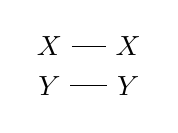
\begin{tikzpicture}
\path (0,0) node (E) {$X$}
++(1,0) node (F) {$X$}
(0,-0.5) node (F1) {$Y$}
+(1,0) node (G) {$Y$};
\draw (E) -- (F);
\draw (F1) -- (G);
\end{tikzpicture}\\
&= 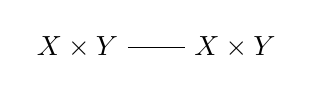
\begin{tikzpicture}
\path (0,0) node (X) {$X\times Y$}
++(2,0) node (Y) {$X\times Y$};
\draw (X) -- (Y);
\end{tikzpicture}
\end{align}

Because a product space can be represented by parallel wires, a kernel $\kernel{L}:X\to \Delta(\mathcal{Y}\otimes\mathcal{Z})$ can be written using either two parallel output wires or a single output wire:

\begin{align}
&\begin{tikzpicture}
\path (0,0) node (E) {$X$}
++ (1,0) node[kernel] (L) {$\kernel{L}$}
++ (1,0.15) node (F) {$Y$}
+(0,-0.3) node (G) {$Z$};
\draw (E) -- (L);
\draw ($(L.east) + (0,0.15)$) -- (F);
\draw ($(L.east)+ (0,-0.15)$) -- (G);
\end{tikzpicture}\\
&\equiv\\
&\begin{tikzpicture}
\path (0,0) node (E) {$X$}
++ (1,0) node[kernel] (L) {$\kernel{L}$}
++ (1.5,0) node (F) {$Y\times Z$};
\draw (E) -- (L) -- (F);
\end{tikzpicture}
\end{align}

\paragraph{Probability measures, Markov kernels and functions}

One has to exercise special care when including functions in diagrammatic notation. While any diagram that includes only probability measures (triangles pointing to the left) and Markov kernels (rectangles) is automatically a Markov kernel itself, while diagrams that include functions (triangles pointing to the right) only represent Markov kernels if they are correctly normalised, which is not a property that can be checked just by looking at the shape of the diagram.

\paragraph{Markov kernels with special notation}

A number of Markov kernels are given special notation distinct from the generic ``box'' representation above. These special representations facilitate intuitive graphical interpretations.

The identity kernel $\textbf{Id}:X\to \Delta(X)$ maps a point $x$ to the measure $\delta_x$ that places all mass on the same point:

\begin{align}
\textbf{Id} : x\mapsto \delta_x \equiv \begin{tikzpicture}\path (0,0) node (X) {$X$} + (1,0) node (X1) {$X$}; \draw (X)--(X1); \end{tikzpicture}\label{eq:identity}
\end{align}

The identity kernel acts as the identity under left or right products:

\begin{align}
	(\kernel{K}\textbf{Id})_w(A) &= \int_X \textbf{Id}_x(A) d\kernel{K}_w (x) \\
							 	 &= \int_X \delta_x(A) d\kernel{K}_w(x)\\
							 	 &= \int_A d\kernel{K}_w(x)\\
							 	 &= \kernel{K}_w(A)\\
	(\textbf{Id}\kernel{K})_w(A) &= \int_X \kernel{K}_x (A) d\textbf{Id}_w(x)\\
								 &= \int_X  \kernel{K}_x(A) d\delta_w(x)\\
								 &= \kernel{K}_w(A)								  
\end{align}

The copy map $\splitter{0.1}:X\to \Delta(\mathcal{X}\times \mathcal{X})$ maps a point $x$ to two identical copies of x:
\begin{align}
 \splitter{0.1}: x\mapsto \delta_{(x,x)} \equiv 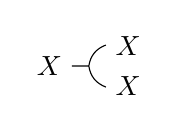
\begin{tikzpicture}
 \path (0,0) node (X) {$X$} ++ (0.5,0) coordinate (copy0) ++ (0.5,0.25) node (X1) {$X$} ++(0,-0.5) node (X2) {$X$};\draw (X)--(copy0) to [bend left] (X1) (copy0) to [bend right] (X2);
 \end{tikzpicture}\label{eq:copy}
 \end{align} 

The copy map ``copies'' its arguments under an integral:

\begin{align}
	\int_(X\times X) f(x,x',x'') d\splitter{0.1}_x (x',x'') &= \int_(X\times X) f(x,x',x'') d\delta_{(x,x)}(x',x'')\\
															&= f(x,x,x)\\
	\int_W \int_(X\times X) f(x',x'')d\splitter{0.1}_w (x',x'') d\mu(w)\\
															&= \int_W f(w,w) d\mu(w)
\end{align}

The swap map $\sigma:X\times Y\to \Delta(\mathcal{Y}\otimes\mathcal{X})$ swaps its inputs:

\begin{align}
\sigma := (x,y)\to \delta_{(y,x)} \equiv 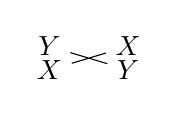
\begin{tikzpicture}
\path (0,0) node (X) {$X$}
+(1,0.3) node (X1) {$X$}
(0,0.3) node (Y) {$Y$}
+(1,-0.3) node (Y1) {$Y$};
\draw (X)--(X1) (Y) -- (Y1);
\end{tikzpicture}\label{eq:swap}
\end{align}

The swap map swaps its arguments under an integral:

\begin{align}
	\int_(X\times X) f(x,x') d\sigma_{(x_0,x_1)}(x,x') &= \int_(X\times X) f(x,x') d\delta_{(x_1,x_0)}(x,x')\\
													   &= f(x_1,x_0)
\end{align}

The discard map $\stopper{0.2}:X\to \Delta(\{*\})$ maps every input to $\delta_{*}$. Note that the only non-empty event in $\{\emptyset,\{*\}\}$ must have probability 1.
\begin{align}
\stopper{0.2}: x\mapsto \delta_{*} \equiv \begin{tikzpicture}
 \draw[-{Rays [n=8]}] (0,0) node (X) {$X$} (X) -- (1,0);
\end{tikzpicture}\label{eq:discard}
\end{align}

Any measurable function $F\to X$ has an associated Markov kernel $F\to \Delta(\mathcal{X})$. The Markov kernel associated with a function is different to the function itself - while the product of a probability measure $\mu$ with a function $f$ is an expectation $\mu f$ (see Definition \ref{def:diag_expectation}), the product of a probability measure with the associated Markov kernel is the pushforward measure $f_\# \mu$.

\begin{definition}[Function induced kernel]\label{def:functional_kernel}
Given a measurable function $g:F\to X$, define the function induced kernel $\kernel{F}^{g}:F\to \Delta(\mathcal{X})$ to be the the Markov kernel $a\mapsto \delta_{g(a)}$ for all $a\in X$.
\end{definition}

\begin{definition}[Pushforward kernel]
Given a kernel $\kernel{M}:E\to \Delta(\mathcal{F})$ and a measurable function $g:F\to X$, the \emph{pushforward kernel} $g_\# \kernel{M}:E\to \Delta(\mathcal{X})$ is the kernel such that $g_\# \kernel{M} (a;B) = \kernel{M}(a;g^{-1}(B))$.

If $E$ is the one element space $\{*\}$, then $\kernel{M}:\{*\}\to \Delta(\mathcal{F})$ can be identified with the probability measure $\kernel{M}_*$ and the pushforward kernel $g_{\#}\kernel{M}$ identified with the pushforward measure $g_{\#} \kernel{M}_*$, so pushforward kernels reduce to pushforward measures.
\end{definition}

\begin{lemma}[Pushforward kernels are functional kernel products]\label{lem:pushf_funk}
Given a kernel $\kernel{M}:E\to \Delta(\mathcal{F})$ and a measurable function $g:F\to X$,the pushforward $g_\# \kernel{M} = \kernel{M} \kernel{F}^{g}$.
\end{lemma}

\begin{proof}
\begin{align}
	\kernel{M}\kernel{F}^g(a;B) &= \int_F \delta_{g(y)}(B) d\kernel{M}_a(y)\\
								&= \int_F \delta_{y}(g^{-1}(B)) d\kernel{M}_a(y)\\
								&= \int_{g^{-1}(B)} d\kernel{M}_a(y)\\
								&= g_{\#} \kernel{M} (a;B)
\end{align}
\end{proof}


\subsubsection{Comparison of notations}

We are in a position to compare the three introduced notations using a few examples. Given $\mu\in\Delta(X),\kernel{A}:X\to \Delta(Y)$ and $A\in \mathcal{X}$, $B\in\mathcal{Y}$, the following correspondences hold, where we express the same object in elementary notation, product notation and string notation respectively:

\begin{align}
\nu:=A\times B\mapsto \int_A A(x;B)d\mu(x) \equiv \mu \splitter{0.1}(\textbf{Id}_X\otimes \kernel{A}) \equiv  \begin{tikzpicture}
\path (0,0) node[dist] (mu) {$\mu$}
++ (1,0) coordinate (copy0)
+ (1.2,0.5) node (X) {$X$}
++ (0.5,-0.5) node[kernel] (A) {$\kernel{A}$}
++(0.7,0) node (Y) {$Y$};
\draw (mu)--(copy0);
\draw (copy0) to [bend left] (X);
\draw (copy0) to [bend right] (A) (A) -- (Y);
\end{tikzpicture}\label{eq:joint_measure}
\end{align}

Where the resulting object is a probability measure $\nu\in \Delta(\mathcal{X}\otimes\mathcal{Y})$. Note that the elementary notation requires a function definition here, while the product and string notations can represent the measure without explicitly addressing its action on various inputs and outputs. \citet{cho_disintegration_2019} calls this construction ``integrating $\kernel{A}$ with respect to $\mu$''.

Define the marginal $\nu_Y\in \Delta(\mathcal{Y}):B\mapsto \nu(X\times B)$ for $B\in \mathcal{Y}$ and similarly for $\nu_X$. We can then express the result of marginalising \ref{eq:joint_measure} over $X$ in our three separate notations as follows:
\begin{align}
  \nu_Y (B) &= \nu(X\times B) = \int_X A(x;B) d\mu(x)\label{eq:marginalisation_elem}\\
  \nu_Y &= \mu \kernel{A} = \mu \splitter{0.1}(\textbf{Id}_X\otimes \kernel{A})(\stopper{0.2}\otimes \textbf{Id}_Y)\label{eq:marginalisation_prod}\\
  \nu_Y &= \begin{tikzpicture}
\path (0,0) node[dist] (mu) {$\mu$} ++ (1,0) node[kernel] (A) {$\kernel{A}$} ++ (0.7,0) node (Y) {$Y$}; \draw (mu) -- (A) -- (Y);
\end{tikzpicture} = \begin{tikzpicture}
\path (0,0) node[dist] (mu) {$\mu$}
++ (1,0) coordinate (copy0)
+ (1.2,0.5) node (X) {}
++ (0.5,-0.5) node[kernel] (A) {$\kernel{A}$}
++(0.7,0) node (Y) {$Y$};
\draw (mu)--(copy0);
\draw[-{Rays [n=8]}] (copy0) to [bend left] (X);
\draw (copy0) to [bend right] (A) (A) -- (Y);
\end{tikzpicture}\label{eq:marginalisation_graph}
\end{align}

The elementary notation \ref{eq:marginalisation_elem} makes the relationship between $\nu_Y$ and $\nu$ explicit and, again, requires the action on each event to be defined. The product notation \ref{eq:marginalisation_prod} is, in my view, the least transparent but also the most compact in the form $\mu \kernel{A}$, and does not demand the explicit definition of how $\nu_Y$ treats every event. The graphical notation is the least compact in terms of space taken up on the page, but unlike the product notation it shows a clear relationship to the graphical construction in\ref{eq:joint_measure}, and displays a clear graphical logic whereby marginalisation corresponds to ``cutting off branches''. Like product notation, it also allows for the definition of derived measures such as $\nu_Y$ without explicit definition of the handling of all events. It also features a much smaller collection of symbols than does elementary notation.

String diagrams often achieve a good balance between being ease of understanding at a glance and expressive power. On the downside, they can be time consuming to typeset, and formal reasoning with them takes some practice.

\subsubsection{Working With String Diagrams}\label{sssec:string_diagram_manipulation}

todo:
\begin{itemize}
\item Functional generalisation
\item Conditioning
\item Infinite copy map
\item De Finetti's representation theorem
\end{itemize}

There are a relatively small number of manipulation rules that are useful for string diagrams. In addition, we will define graphically analogues of the standard notions of \emph{conditional probability}, \emph{conditioning}, and infinite sequences of exchangeable random variables.

\paragraph{Axioms of Symmetric Monoidal Categories}

For the following, we either omit labels or label diagrams with their domain and codomain spaces, as we are discussing identities of kernels rather than identities of components of a condtional probability space. Recalling the unique Markov kernels defined above, the following equivalences, known as the \emph{commutative comonoid axioms}, hold among string diagrams:

\begin{align}
	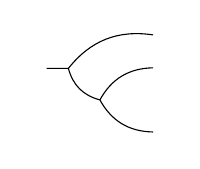
\begin{tikzpicture}[scale=0.8]
	\path (0,0) node (X) {} 
	++ (0.5,0) coordinate (copy0)
	+ (1.5,0.5) node (X1) {}
	++ (0.5,-0.5) coordinate (copy1)
	+(1,0.5) node (X2) {}
	+(1,-0.5) node (X3) {};
	\draw (X) -- (copy0) to [bend left] (X1) (copy0) to [bend right] (copy1) to [bend left] (X2) (copy1) to [bend right] (X3);
	\end{tikzpicture}
	=
	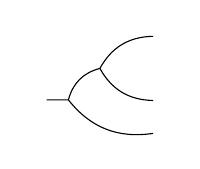
\begin{tikzpicture}[scale=0.8]
	\path (0,0) node (X) {} 
	++ (0.5,0) coordinate (copy0)
	+ (1.5,-0.5) node (X1) {}
	++ (0.5,0.5) coordinate (copy1)
	+(1,0.5) node (X2) {}
	+(1,-0.5) node (X3) {};
	\draw (X) -- (copy0) to [bend right] (X1) (copy0) to [bend left] (copy1) to [bend left] (X2) (copy1) to [bend right] (X3);
	\end{tikzpicture}
	:=
	\begin{tikzpicture}[scale=0.8]
	\path (0,0) node (X) {} 
	++ (0.5,0) coordinate (copy0)
	+ (1,0.5) node (X1) {}
	+(1,0) node (X2) {}
	+(1,-0.5) node (X3) {};
	\draw (X) -- (copy0) to [bend left] (X1) (copy0) to (X2) (copy0) to [bend right] (X3);
	\end{tikzpicture}\label{eq:ccom1}
\end{align}

\begin{align}
	\begin{tikzpicture}[scale=0.8]
	\path (0,0) node (X) {}
	++(0.5,0) coordinate (copy0)
	+ (1,0.5) node (S) {}
	+(1,-0.5) node (X1) {};
	\draw (X) -- (copy0) to [bend right] (X1);
	\draw[-{Rays [n=8]}] (copy0) to [bend left] (S);
	\end{tikzpicture}
	= 
	\begin{tikzpicture}[scale=0.8]
	\path (0,0) node (X) {}
	++(0.5,0) coordinate (copy0)
	+ (1,-0.5) node (S) {}
	+(1,0.5) node (X1) {};
	\draw (X) -- (copy0) to [bend left] (X1);
	\draw[-{Rays [n=8]}] (copy0) to [bend right] (S);
	\end{tikzpicture}
	=
	\begin{tikzpicture}[scale=0.8]
	\path (0,0) node (X) {}
	++ (1,0) node (X1) {};
	\draw (X) -- (X1);
	\end{tikzpicture}\label{eq:ccom2}
\end{align}

\begin{align}
	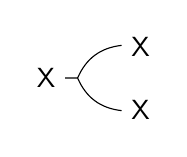
\begin{tikzpicture}[scale=0.8]
	\path (0,0) node (X) {$\RV{X}$}
	++(0.5,0) coordinate (copy0)
	+ (1,0.5) node (X2) {$\RV{X}$}
	+(1,-0.5) node (X1) {$\RV{X}$};
	\draw (X) -- (copy0) to [bend right] (X1);
	\draw (copy0) to [bend left] (X2);
	\end{tikzpicture}
=
	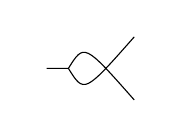
\begin{tikzpicture}[scale=0.8]
	\path (0,0) node (X) {}
	++(0.5,0) coordinate (copy0)
	+ (1.2,0.5) node (X2) {}
	+(1.2,-0.5) node (X1) {};
	\draw (X) -- (copy0) .. controls (0.75,0.4) .. (X1.west);
	\draw (copy0) .. controls (0.75,-0.4) .. (X2.west);
	\end{tikzpicture}
\label{eq:ccom3}
\end{align}

The discard map $\stopper{0.2}$ can ``fall through'' any Markov kernel:

\begin{align}
\begin{tikzpicture}
\path (0,0) node (X) {}
++(0.7,0) node[kernel] (A) {$\kernel{A}$}
++(0.7,0) node (S) {};
\draw (X) -- (A);
\draw[-{Rays [n=8]}] (A) -- (S);
\end{tikzpicture}
= 
\begin{tikzpicture}
\path (0,0) node (X) {}
++(0.7,0) node (S) {};
\draw[-{Rays [n=8]}] (X) -- (S);
\end{tikzpicture}\label{eq:termobj1}
\end{align}

Combining \ref{eq:ccom2} and \ref{eq:termobj1} we can derive the following: integrating $\kernel{A}:X\to \Delta(\mathcal{Y})$ with respect to $\mu\in\Delta(\mathcal{X})$ and then discarding the output of $\kernel{A}$ leaves us with $\mu$:

\begin{align}
\begin{tikzpicture}
\path (0,0) node[dist] (mu) {$\mu$}
++ (1,0) coordinate (copy0)
+ (1.4,0.5) node (X) {}
++ (0.7,-0.5) node[kernel] (A) {$\kernel{A}$}
++(0.7,0) node (Y) {};
\draw (mu)--(copy0);
\draw (copy0) to [bend left] (X);
\draw[-{Rays [n=8]}] (copy0) to [bend right] (A) (A) -- (Y);
\end{tikzpicture}
= 
\begin{tikzpicture}
\path (0,0) node[dist] (mu) {$\mu$}
++ (1,0) coordinate (copy0)
+ (1.2,0.5) node (X) {}
++ (0.4,-0.3) coordinate (A)
++(0.1,0) node (Y) {};
\draw (mu)--(copy0);
\draw (copy0) to [bend left] (X);
\draw[-{Rays [n=8]}] (copy0) to [bend right] (A) (A) -- (Y);
\end{tikzpicture}
=
\begin{tikzpicture}
\path (0,0) node[dist] (mu) {$\mu$}
++ (1,0) node (X) {};
\draw (mu)--(X);
\end{tikzpicture}
\end{align}

In elementary notation, this is equivalent to the fact that, for all $B\in \mathcal{X}$, $\int_B \kernel{A}(x;B)d\mu(x) = \mu(B)$.

The following additional properties hold for $\stopper{0.2}$ and $\splitter{0.1}$:

\begin{align}
\begin{tikzpicture}
\path (0,0) node (XY) {$X\times Y$}
++ (1.5,0) node (Z) {};
\draw[-{Rays [n=8]}] (XY) -- (Z);
\end{tikzpicture} &=
\begin{tikzpicture}
\path (0,0) node (X) {$X$} 
++ (1,0) node (X1) {}
(0,-0.3) node (Y) {$Y$}
++ (1,0) node (Y1) {};
\draw[-{Rays [n=8]}] (X) -- (X1);
\draw[-{Rays [n=8]}] (Y) -- (Y1);
\end{tikzpicture}
\end{align}
\begin{align}
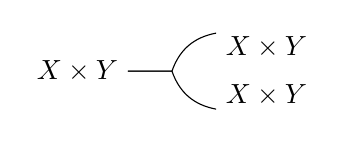
\begin{tikzpicture}
\path (0,0) node (XY) {$X\times Y$}
++ (1.2,0) coordinate (copy0)
++(1.2,0.3) node (XY1) {$X \times Y$}
++(0,-0.6) node (XY2) {$X\times Y$};
\draw (XY) -- (copy0) to [bend left] (XY1);
\draw (XY) -- (copy0) to [bend right] (XY2);
\end{tikzpicture} &=
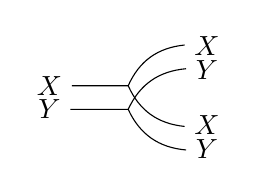
\begin{tikzpicture}
\path (0,0) node (XY) {$X$}
++ (1.,0) coordinate (copy0)
++(1.,0.5) node (XY1) {$X$}
++(0,-1) node (XY2) {$X$}
(0,-0.3) node (F) {$Y$}
++(1.,0) coordinate (copy1)
++(1.,0.5) node (F1) {$Y$}
++(0,-1) node (F2) {$Y$};
\draw (XY) -- (copy0) to [bend left] (XY1);
\draw (copy0) to [bend right] (XY2);
\draw (F) -- (copy1) to [bend left] (F1);
\draw (copy1) to [bend right] (F2);
\end{tikzpicture}
\end{align}

A key fact that \emph{does not} hold in general is

\begin{align}
 \begin{tikzpicture}
\path (0,0) node (E) {}
++ (0.7,0) node[kernel] (A) {$\kernel{A}$}
++(0.7,0) coordinate (copy0)
++(0.5,0.3) node (F1) {}
+(0,-0.6) node (F2) {};
\draw (E) -- (A) -- (copy0) to [bend left] (F1);
\draw (copy0) to [bend right] (F2);
\end{tikzpicture} 
=
\begin{tikzpicture}
\path (0,0) node (E) {}
++(0.5,0) coordinate (copy0)
++(0.7,0.3) node[kernel] (A1) {$\kernel{A}$}
+(0,-0.6) node[kernel] (A2) {$\kernel{A}$}
++(0.75,0) node (F1) {}
+(0,-0.6) node (F2) {};
\draw (E) -- (copy0) to [bend left] (A1) (A1) -- (F1);
\draw (copy0) to [bend right] (A2) (A2) -- (F2);
\end{tikzpicture}
\label{eq:copy_commutes}
\end{align}

In fact, it holds only when $\kernel{A}$ is a \emph{deterministic} kernel.

\begin{definition}[Deterministic Markov kernel]
A \emph{deterministic} Markov kernel $\kernel{A}:E\to \Delta(\mathcal{F})$ is a kernel such that $\kernel{A}_x(B)\in\{0,1\}$ for all $x\in E$, $B\in\mathcal{F}$.
\end{definition}

\begin{theorem}[Copy map commutes for deterministic kernels \citep{fong_causal_2013}]
Equation \ref{eq:copy_commutes} holds iff $\kernel{A}$ is deterministic.
\end{theorem}


\subsection{Random Variables}\label{ssec:random_variables}

The summary of this section is:
\begin{itemize}
\item Random variables are usually defined as measurable functions on a \emph{probability space}
\item It's possible to define them as measurable functions on a \emph{Markov kernel space} instead
\item It is useful to label wires with random variable names instead of names of spaces
\end{itemize}

Probability theory is primarily concerned with the behaviour of \emph{random variables}. This behaviour can be analysed via a collection of probability measures and Markov kernels representing joint, marginal and conditional distributions of random variables of interest. In the framework developed by Kolmogorov, this collection of joint, marginal and conditional distributions is modeled by a single underlying \emph{probability space}, and random variables by measurable functions on the probability space. 

We use the same approach here, with a couple of additions. We are interested in variables whose outcomes depend both on random processes and decisions. Suppose that given a particular distribution over decision variables, a probability distribution over the decision variables and random variables is obtained. Such a model is described by a Markov kernel rather than a probability distribution. We therefore investigate \emph{Markov kernel spaces}.

In the graphical notation that we are using, random variables can be thought of as a means of assigning unambiguous names to each wire in a set of diagrams. In order to do this, it is necessary to suppose that all diagrams in the set describe properties of an \emph{ambient Markov kernel} or \emph{ambient probability measure}. Consider the following example with the ambient probability measure $\mu\in\Delta(\mathcal{X}\otimes\mathcal{X})$. Suppose we have a Markov kernel $\kernel{K}:X\to \Delta(\mathcal{X})$ such that the following holds:

\begin{align}
\begin{tikzpicture}
\path (0,0) node[dist] (m) {$\mu$}
++ (0.7,0.15) node (E) {$X$}
++ (0,-0.3) node (F) {$X$};
\draw ($(m.east) + (0,0.15)$) -- (E);
\draw ($(m.east) + (0,-0.15)$) -- (F);
\end{tikzpicture} = \begin{tikzpicture}
\path (0,0) node[dist] (m) {$\mu$}
++ (0.7,0.15) coordinate (copy0)
+(0,-0.3) node (Fs) {}
++ (1.2,0) node (E) {$X$}
++(-0.7,-0.3) node[kernel] (K) {$\kernel{K}$}
++(0.7,0) node (F) {$X$};
\draw ($(m.east) + (0,0.15)$) -- (E);
\draw (copy0) to [bend right] (K) (K) -- (F);
\draw[-{Rays [n=8]}] ($(m.east) + (0,-0.15)$) -- (Fs);
\end{tikzpicture}\label{eq:disint_example}
\end{align}

Suppose that we also assign the names $\RV{X}_1$ to the upper output wire and $\RV{X}_2$ to the lower output wire in the diagram of $\mu$:

\begin{align}
\begin{tikzpicture}
\path (0,0) node[dist] (m) {$\mu$}
++ (0.7,0.15) node (E) {$\RV{X}_1$}
++ (0,-0.3) node (F) {$\RV{X}_2$};
\draw ($(m.east) + (0,0.15)$) -- (E);
\draw ($(m.east) + (0,-0.15)$) -- (F);
\end{tikzpicture}
\end{align}

Then it seems sensible to call $\kernel{K}$ ``the probability of $\RV{X}_2$ given $\RV{X}_1$''. We will make this precise so that it matches the usual notion of the probability of one variable given another (see \citet{cinlar_probability_2011} for a definition of this usual notion). 

\begin{definition}[Probability space, Markov kernel space]
A \emph{Markov kernel space} $(\kernel{K},\Omega,\mathcal{F},D,\mathcal{D})$ is a Markov kernel $\kernel{K}:D\to \Delta(\mathcal{D}\otimes\mathcal{F})$, called the \emph{ambient kernel}, along with the sample space $(\Omega,\mathcal{F})$ and the domain $(D,\mathcal{D})$. We suppose that $\kernel{K}$ is such that there exists a \emph{fundamental kernel} $\kernel{K}_0$ satisfying

\begin{align}
\prob{K} := \begin{tikzpicture}
\path (0,0) node (O) {}
++(0.5,0) coordinate (copy0)
++ (0.5,0) node[kernel] (m) {$\kernel{K}_0$}
++ (0.7,0.) node (E) {}
++(0,-0.45) node (G) {};
\draw (O) -- (m) -- (E);
\draw (copy0) to [bend right] (G);
\end{tikzpicture}
\end{align}

For brevity, we will omit the $\sigma$-algebras in further definitions of Markov kernel spaces: $(\kernel{K},\Omega,D)$.

A \emph{probability space} $(\prob{P},\Omega,\mathcal{F})$ is a probability measure $\prob{P}:\Delta(\Omega)$, which we call the \emph{ambient measure}, along with the \emph{sample space} $\Omega$ and the \emph{events} $\mathcal{F}$. A probability space is equivalent to a Markov kernel space with domain $D=\{*\}$ - note that $\Omega\times \{*\}\cong \Omega$.
\end{definition}

\begin{definition}[Random variable]\label{def:random_variable}
Given a Markov kernel space $(\kernel{K},\Omega,D)$, a random variable $\RV{X}$ is a measurable function $\Omega\times D\to E$ for arbitrary measurable $E$.
\end{definition}

\begin{definition}[Domain variable]\label{def:domain_variable}
Given a Markov kernel space $(\kernel{K},\Omega,D)$, the \emph{domain variable} $\RV{D}:\Omega\times D\to D$ is the distinguished random variable $\RV{D}:(x,d)\mapsto d$.
\end{definition}

Unlike random variables on probability spaces, random variables on Markov kernel spaces do not generally have unique marginal distributions. An analogous operation of \emph{marginalisation} can be defined, but the result is generally a Markov kernel. We will define marginalisation via coupled tensor products.

\begin{definition}[Coupled tensor product $\utimes$]\label{def:ctensor}
Given two Markov kernels $\kernel{M}$ and $\kernel{N}$ or functions $f$ and $g$ with shared domain $E$, let $\kernel{M}\utimes\kernel{N}:=\splitter{0.1}(\kernel{M}\otimes\kernel{N})$ and $f\utimes g:=\splitter{0.1}(f\otimes g)$ where these expressions are interpreted using standard product notation. Graphically:

\begin{align}
\kernel{M}\utimes\kernel{N}&:=\begin{tikzpicture}
\path (0,0) node (E) {$E$}
++(0.5,0) coordinate (copy0)
+ (0.5,0.3) node[kernel] (M) {$\kernel{M}$}
+(1.2,0.3) node (X) {$\RV{X}$}
+ (0.5,-0.3) node[kernel] (N) {$\kernel{N}$}
+(1.2,-0.3) node (Y) {$\RV{Y}$};
\draw (E) -- (copy0) to [bend left] (M) (copy0) to [bend right] (N);
\draw (M) -- (X) (N) -- (Y);
\end{tikzpicture}\\
f\utimes g&:= \begin{tikzpicture}[scale=1.2]\path (0,0) node (E) {$E$}
++(0.5,0) coordinate (copy0)
+ (0.5,0.3) node[expectation] (M) {$f$}
+ (0.5,-0.3) node[expectation] (N) {$g$};
\draw (E) -- (copy0) to [bend left] (M) (copy0) to [bend right] (N);
\end{tikzpicture}
\end{align}
The operation denoted by $\utimes$ is associative (Lemma \ref{lem:utimes_assoc}), so we can without ambiguity write $f\utimes g\utimes h=(f\utimes g)\utimes h = f\utimes(g\utimes h)$ for finite groups of functions or Markov kernels sharing a domain. 

The notation $\utimes_{i\in [N]} f_i$ is taken to mean $f_1\utimes f_2\utimes ...\utimes f_N$.
\end{definition}

\begin{lemma}[$\utimes$ is associative]\label{lem:utimes_assoc}
For Markov kernels $\kernel{L}:E\to \delta(\mathcal{F})$, $\kernel{M}:E\to \delta(\mathcal{G})$ and $\kernel{N}:E\to \delta(\mathcal{H})$, $(\kernel{L}\utimes\kernel{M})\utimes\kernel{N}=\kernel{L}\utimes(\kernel{M}\utimes\kernel{N})$.
\end{lemma}

\begin{proof}

\begin{align}
	\kernel{L}\utimes(\kernel{M}\utimes\kernel{N}) &= 
	\begin{tikzpicture}[scale=0.8]
	\path (0,0) node (X) {$E$} 
	++ (0.8,0) coordinate (copy0)
	+ (1.5,0.5) node[kernel] (X1) {$\kernel{L}$} + (2.5,0.5) node (F) {$F$}
	++ (0.5,-0.5) coordinate (copy1)
	+(1,0.3) node[kernel] (X2) {$\kernel{M}$} + (2,0.3) node (G) {$G$}
	+(1,-0.5) node[kernel] (X3) {$\kernel{N}$} + (2,-0.5) node (H) {$H$};
	\draw (X) -- (copy0) to [bend left] (X1) (copy0) to [bend right] (copy1) to [bend left] (X2) (copy1) to [bend right] (X3);
	\draw (X1) -- (F) (X2) -- (G) (X3) -- (H);
	\end{tikzpicture}\\
	&=
	\begin{tikzpicture}[scale=0.8]
	\path (0,0) node (X) {$E$} 
	++ (0.8,0) coordinate (copy0)
	+ (1.5,0.7) node[kernel] (X1) {$\kernel{L}$} + (2.5,0.7) node (F) {$F$}
	+ (0.5,0.3) coordinate (copy1)
	++ (0.5,-0.5) coordinate (next)
	+(1,0.5) node[kernel] (X2) {$\kernel{M}$} + (2,0.5) node (G) {$G$}
	+(1,-0.5) node[kernel] (X3) {$\kernel{N}$} + (2,-0.5) node (H) {$H$};
	\draw (X) -- (copy0) to [bend left] (copy1) (copy0) to [bend right] (X3);
	\draw (copy1) to [bend left] (X1) (copy1) to [bend right] (X2);
	\draw (X1) -- (F) (X2) -- (G) (X3) -- (H);
	\end{tikzpicture}\\
	&= (\kernel{L}\utimes\kernel{M})\utimes\kernel{N}
\end{align}
This follows directly from Equation \ref{eq:ccom1}.
\end{proof}

\begin{definition}[Marginal distribution, marginal kernel]\label{def:marginal_distribution}
Given a probability space $(\prob{P},\Omega,\mathcal{F})$ and the random variable $\RV{X}:\Omega\to G$ the \emph{marginal distribution} of $\RV{X}$ is the probability measure $\prob{P}^{\RV{X}}:= \prob{P}\kernel{F}^{\RV{X}}$.

See Lemma \ref{lem:pushf_funk} for the proof that this matches the usual definition of marginal distribution.

Given a Markov kernel space $(\kernel{K},\Omega,\mathcal{F},D,\mathcal{D})$ and the random variable $\RV{X}:\Omega\to G$, the \emph{marginal kernel} is $\kernel{K}^{\RV{X}|\RV{D}}:=\kernel{K}\kernel{F}^{\RV{X}}$.
\end{definition}

\begin{definition}[Joint distribution, joint kernel]\label{def:joint_distribution}
Given a probability space $(\prob{P},\Omega,\mathcal{F})$ and the random variables $\RV{X}:\Omega\to G$ and $\RV{Y}:\Omega\to H$, the \emph{joint distribution} of $\RV{X}$ and $\RV{Y}$, $\prob{P}^{\RV{X}\RV{Y}}\in \Delta(\mathcal{G}\otimes\mathcal{H})$, is the marginal distribution of $\RV{X}\utimes\RV{Y}$. That is, $\prob{P}^{\RV{X}\RV{Y}}:=\prob{P} \kernel{F}^{\RV{X}\utimes\RV{Y}}$

This is identical to the definition in \citet{cinlar_probability_2011} if we note that the random variable $(\RV{X},\RV{Y}):\omega\mapsto (\RV{X}(\omega),\RV{Y}(\omega))$ (\c{C}inlar's definition) is precisely the same thing as $\RV{X}\utimes\RV{Y}$.

Analogously, the joint kernel $\kernel{K}^{\RV{X}\RV{Y}|\RV{D}}$ is the product $\kernel{K}\kernel{F}^{\RV{X}\utimes\RV{Y}}$.
\end{definition}

Joint distributions and kernels have a nice visual representation, as a result of Lemma \ref{lem:jdist_cprod} which follows.

\begin{lemma}[Product marginalisation interchange]\label{lem:jdist_cprod}
Given two functions, the kernel associated with their coupled product is equal to the coupled product of the kernels associated with each function.

Given $\RV{X}:\Omega\to G$ and $\RV{Y}:\Omega\to H$, $\kernel{F}^{\RV{X}\utimes\RV{Y}}=\kernel{F}^\RV{X}\utimes\kernel{F}^\RV{Y}$
\end{lemma}

\begin{proof}
For $a\in \Omega$, $B\in \mathcal{G}$, $C\in \mathcal{H}$,
\begin{align}
\kernel{F}^{\RV{X}\utimes\RV{Y}} (a;B\times C) &= \delta_{\RV{X}(a),\RV{Y}(a)}(B\times C)\\
									   &= \delta_{\RV{X}(a)}(B)\delta_{\RV{Y}(a)}(C)\\
									   &= (\delta_{\RV{X}(a)}\otimes\delta_{\RV{Y}(a)})(B\times C)\\
									   &= \kernel{F}^{\RV{X}}\utimes\kernel{F}^{\RV{Y}}
\end{align}
Equality follows from the monotone class theorem.
\end{proof}

\begin{corollary}\label{corr:rewrite_joint_dist}
Given a Markov kernel space $(\kernel{K}, \Omega, D)$ and random variables $\RV{X}:\Omega\times D\to X$, $\RV{Y}:\Omega\times D\to Y$, the following holds:

\begin{align}
\begin{tikzpicture}
\path (0,0) node (O) {$D$}
++(1,0) node[kernel] (K) {$\kernel{K}^{\RV{X}\RV{Y}|\RV{D}}$}
++ (1,0.15) node (X) {$X$}
+(0,-0.3) node (Y) {$Y$};
\draw (O) -- (K);
\draw ($(K.east) + (0,0.15)$) -- (X);
\draw ($(K.east) + (0,-0.15)$) -- (Y);
\end{tikzpicture}=
\begin{tikzpicture}
\path (0,0) node (O) {$D$}
++ (0.7, 0) node[kernel] (K) {$\kernel{K}$}
++ (0.6,0) coordinate (copy0)
++ (0.4,0.25) node[kernel] (X) {$\kernel{F}^{\RV{X}}$}
+(0,-0.5) node[kernel] (Y) {$\kernel{F}^{\RV{Y}}$}
++(0.7,0) node (Xo) {$X$}
+(0,-0.5) node (Yo) {$Y$};
\draw (O) -- (K) -- (copy0);
\draw (copy0) to [bend left] (X) (X) -- (Xo);
\draw (copy0) to [bend right] (Y) (Y) -- (Yo);
\end{tikzpicture}
\end{align}
\end{corollary}

We will now define wire labels for ``output'' wires.

\begin{definition}[Wire labels - joint kernels]\label{def:wl_jprob}
Suppose we have a Markov kernel space $(\kernel{K},\Omega,D)$, random variables $\RV{X}:\Omega\times D\to X$, $\RV{Y}:\Omega\times D\to Y$ and a Markov kernel $\kernel{L}:D\to \Delta(\mathcal{X}\times\mathcal{Y})$. The following \emph{output labelling} of $\mathbf{L}$:

\begin{align}
\begin{tikzpicture}
\path (0,0) node (A) {$D$}
++ (0.7,0) node[kernel] (m) {$\kernel{L}$}
++ (0.7,0.15) node (E) {\color{blue}$\RV{X}$}
++ (0,-0.3) node (F) {\color{blue}$\RV{Y}$};
\draw (A) -- (m);
\draw ($(m.east) + (0,0.15)$) -- (E);
\draw ($(m.east) + (0,-0.15)$) -- (F);
\end{tikzpicture}
\end{align}

is \emph{valid} iff

\begin{align}
\kernel{L} = \kernel{K}_{\RV{X}\RV{Y}|\RV{D}}\label{eq:labels_express_joint}
\end{align}

and

\begin{align}
\begin{tikzpicture}
\path (0,0) node (A) {$D$}
++ (1,0) node[kernel] (m) {$\kernel{L}$}
++ (1,0.15) node (E) {\color{blue}$\RV{X}$}
++ (0,-0.3) node (F) {};
\draw (A) -- (m) ($(m.east) + (0,0.15)$) -- (E);
\draw[-{Rays [n=8]}] ($(m.east) + (0,-0.15)$) -- (F);
\end{tikzpicture} = \kernel{K}^{\RV{X}|\RV{D}}\label{eq:labels_express_marginal_upper}
\end{align}

and

\begin{align}
\begin{tikzpicture}
\path (0,0) node (A) {$D$}
++ (1,0) node[kernel] (m) {$\kernel{L}$}
++ (1,0.15) node (E) {}
++ (0,-0.3) node (F) {\color{blue}$\RV{Y}$};
\draw (A) -- (m);
\draw[-{Rays [n=8]}] ($(m.east) + (0,0.15)$) -- (E);
\draw ($(m.east) + (0,-0.15)$) -- (F);
\end{tikzpicture} = \kernel{K}^{\RV{Y}|\RV{D}}\label{eq:labels_express_marginal_lower}
\end{align}

The second and third conditions are nontrivial: suppose $\RV{X}$ takes values in some product space $Range(\RV{X}) = W\times Z$, and $\RV{Y}$ takes values in $Y$. Then we could have $\kernel{L}=\kernel{K}^{\RV{X}\RV{Y}|\RV{D}}$ and draw the diagram

\begin{align}
\begin{tikzpicture}
\path (0,0) node (A) {$D$}
++ (0.7,0) node[kernel] (m) {$\kernel{L}$}
++ (1,0.15) node (E) {$W$}
++ (0.3,-0.3) node (F) {$Z\times Y$};
\draw (A) -- (m);
\draw ($(m.east) + (0,0.15)$) -- (E);
\draw ($(m.east) + (0,-0.15)$) -- (F);
\end{tikzpicture}\label{eq:cannot_marginalise}
\end{align}

For \emph{this} diagram, properties \ref{eq:labels_express_marginal_upper} and \ref{eq:labels_express_marginal_lower} do not hold, even though \ref{eq:labels_express_joint} does.

\end{definition}

\begin{lemma}[Output label assignments exist]
Given Markov kernel space $(\kernel{K},\Omega,D)$, random variables $\RV{X}:\Omega\times D\to X$ and $\RV{Y}:\Omega\times D\to Y$ then there exists a diagram of $\kernel{L}:=\kernel{K}^{\RV{X}\RV{Y}|\RV{D}}$ with a valid output labelling assigning ${\color{blue}\RV{X}}$ and ${\color{blue}\RV{Y}}$ to the output wires.
\end{lemma}

\begin{proof}
By definition, $\kernel{L}$ has signature $D\to \Delta(\mathcal{X}\otimes\mathcal{Y})$. Thus, by the rule that tensor product spaces can be represented by parallel wires, we can draw

\begin{align}
\begin{tikzpicture}
\path (0,0) node (A) {$D$}
++ (0.7,0) node[kernel] (m) {$\kernel{L}$}
++ (0.7,0.15) node (E) {$X$}
++ (0,-0.3) node (F) {$Y$};
\draw (A) -- (m);
\draw ($(m.east) + (0,0.15)$) -- (E);
\draw ($(m.east) + (0,-0.15)$) -- (F);
\end{tikzpicture}
\end{align}

By Corollary \ref{corr:rewrite_joint_dist}, we have

\begin{align}
\begin{tikzpicture}
\path (0,0) node (A) {$D$}
++ (0.7,0) node[kernel] (m) {$\kernel{L}$}
++ (0.7,0.15) node (E) {$X$}
++ (0,-0.3) node (F) {$Y$};
\draw (A) -- (m);
\draw ($(m.east) + (0,0.15)$) -- (E);
\draw ($(m.east) + (0,-0.15)$) -- (F);
\end{tikzpicture} = \begin{tikzpicture}
\path (0,0) node (O) {$D$}
++ (0.7, 0) node[kernel] (K) {$\kernel{K}$}
++ (0.6,0) coordinate (copy0)
++ (0.4,0.25) node[kernel] (X) {$\kernel{F}^{\RV{X}}$}
+(0,-0.5) node[kernel] (Y) {$\kernel{F}^{\RV{Y}}$}
++(0.7,0) node (Xo) {$X$}
+(0,-0.5) node (Yo) {$Y$};
\draw (O) -- (K) -- (copy0);
\draw (copy0) to [bend left] (X) (X) -- (Xo);
\draw (copy0) to [bend right] (Y) (Y) -- (Yo);
\end{tikzpicture}
\end{align}

Therefore 

\begin{align}
\begin{tikzpicture}
\path (0,0) node (O) {$D$}
++ (0.7, 0) node[kernel] (K) {$\kernel{K}$}
++ (0.6,0) coordinate (copy0)
++ (0.4,0.25) node[kernel] (X) {$\kernel{F}^{\RV{X}}$}
+(0,-0.5) node[kernel] (Y) {$\kernel{F}^{\RV{Y}}$}
++(0.7,0) node (Xo) {$X$}
+(0,-0.5) node (Yo) {};
\draw (O) -- (K) -- (copy0);
\draw (copy0) to [bend left] (X) (X) -- (Xo);
\draw[-{Rays[n=8]}] (copy0) to [bend right] (Y) (Y) -- (Yo);
\end{tikzpicture} &= \kernel{K}\kernel{F}^{\RV{X}}\\
				 &= \kernel{K}^{\RV{X}|\RV{D}}
\end{align}

\begin{align}
\begin{tikzpicture}
\path (0,0) node (O) {$D$}
++ (0.7, 0) node[kernel] (K) {$\kernel{K}$}
++ (0.6,0) coordinate (copy0)
++ (0.4,0.25) node[kernel] (X) {$\kernel{F}^{\RV{X}}$}
+(0,-0.5) node[kernel] (Y) {$\kernel{F}^{\RV{Y}}$}
++(0.7,0) node (Xo) {}
+(0,-0.5) node (Yo) {$Y$};
\draw (O) -- (K) -- (copy0);
\draw[-{Rays[n=8]}] (copy0) to [bend left] (X) (X) -- (Xo);
\draw (copy0) to [bend right] (Y) (Y) -- (Yo);
\end{tikzpicture} &= \kernel{K}\kernel{F}^{\RV{Y}}\\
				 &= \kernel{K}^{\RV{Y}|\RV{D}}
\end{align}
\end{proof}

In all further work, wire labels will be used without special colouring.

\begin{definition}[Disintegration]\label{def:disintegration}
Given a probability space $(\prob{P},\Omega,\mathcal{F})$, and random variables $\RV{X}$ and $\RV{Y}$, we say that $\kernel{M}:E\to \Delta(\mathcal{F})$ is a \emph{$\RV{Y}$ on $\RV{X}$ disintegration} of $\prob{P}$ iff
\begin{align}
\begin{tikzpicture}
\path (0,0) node[dist] (m) {$\prob{P}^{\RV{X}\RV{Y}}$}
++ (1,0.15) node (E) {$\RV{X}$}
++ (0,-0.3) node (F) {$\RV{Y}$};
\draw ($(m.east) + (0,0.15)$) -- (E);
\draw ($(m.east) + (0,-0.15)$) -- (F);
\end{tikzpicture} = \begin{tikzpicture}
\path (0,0) node[dist] (m) {$\prob{P}^{\RV{X}}$}
++ (0.7,0.15) coordinate (copy0)
+(0.2,-0.3) node (T) {}
++ (1.2,0) node (E) {$\RV{X}$}
++(-0.7,-0.3) node[kernel] (K) {$\kernel{M}$}
++(0.7,0) node (F) {$\RV{Y}$};
\draw ($(m.east) + (0,0.15)$) -- (E);
\draw (copy0) to [bend right] (K) (K) -- (F);
\draw[-{Rays [n=8]}] ($(m.east) + (0,-0.15)$) -- (T);
\end{tikzpicture}\label{eq:ordinary_disint}
\end{align}
$\kernel{M}$ is a version of $\prob{P}^{\RV{Y}|\RV{X}}$, ``the probability of $\RV{Y}$ given $\RV{X}$''. Let $\prob{P}^{\{\RV{Y}|\RV{X}\}}$ be the set of all kernels that satisfy \ref{eq:ordinary_disint} and $\prob{P}^{\RV{Y}|\RV{X}}$ an arbitrary member of $\prob{P}^{\RV{Y}|\RV{X}}$.

Given a Markov kernel space $(\kernel{K},\Omega,D)$ and random variables $\RV{X}:\Omega\times D\to X$, $\RV{Y}:\Omega\times D\to Y$, $\kernel{M}:D\times E\to \Delta(\mathcal{F})$ is a \emph{$\RV{Y}$ on $\RV{DX}$ disintegration} of $\kernel{K}^{\RV{YX}|\RV{D}}$ iff

\begin{align}
\begin{tikzpicture}
\path (0,0) node (O) {}
++ (1,0) node[kernel] (m) {$\kernel{K}^{\RV{YX}|\RV{D}}$}
++ (1,0.15) node (E) {$\RV{X}$}
++ (0,-0.3) node (F) {$\RV{Y}$};
\draw (O) -- (m) ($(m.east) + (0,0.15)$) -- (E);
\draw ($(m.east) + (0,-0.15)$) -- (F);
\end{tikzpicture} = \begin{tikzpicture}
\path (0,0) node (O) {}
++ (0.3,0) coordinate (copy1)
++ (1,0) node[kernel] (m) {$\kernel{K}^{\RV{YX}|\RV{D}}$}
++ (1,0.15) coordinate (copy0)
+(0.2,-0.3) node (T) {}
++ (1.2,0) node (E) {$\RV{X}$}
++(-0.7,-0.3) node[kernel] (K) {$\kernel{M}$}
++(0.7,0) node (F) {$\RV{Y}$};
\draw (O) -- (m) ($(m.east) + (0,0.15)$) -- (E);
\draw (copy0) to [bend right] (K) (K) -- (F);
\draw (copy1) to [out=290,in=180] ($(K.west) + (0,-0.15)$);
\draw[-{Rays [n=8]}] ($(m.east) + (0,-0.15)$) -- (T);
\end{tikzpicture}\label{eq:def_k_disint}
\end{align}

Write $\kernel{K}^{\{\RV{Y}|\RV{XD}\}}$ for the set of kernels satisfying \ref{eq:def_k_disint} and $\kernel{K}^{\RV{Y}|\RV{XD}}$ for an arbitrary member of $\kernel{K}^{\{\RV{Y}|\RV{XD}\}}$.
\end{definition}

\begin{definition}[Wire labels -- input]\label{def:wl_disint}

An input wire is \emph{connected} to an output wire if it is possible to trace a path from the start of the input wire to the end of the output wire without passing through any boxes, erase maps or right facing triangles.

If an input wire is connected to an output wire and that output wire has a valid label $\RV{X}$, then it is valid to label the input wire with $\RV{X}$.

For example, if the following are valid output labels with respect to $(\prob{P},\Omega)$:

\begin{align}
\begin{tikzpicture}
\path (0,0) node (A) {}
++ (0.7,0) coordinate (copy0)
++ (0.7,0) node[kernel] (m) {$\kernel{L}$}
++ (0.7,0) node (E) {\color{blue}$\RV{X}$}
++ (0,-0.3) node (F) {\color{blue}$\RV{Y}$};
\draw (A) -- (m) -- (E);
\draw (copy0) to [out=-60,in=180] (F);
\end{tikzpicture}\label{dia:kernel_l}
\end{align}

i.e. if $\kernel{L}\in \prob{P}^{\{\RV{X}\RV{Y}|\RV{Y}\}}$, then the following is a valid input label:


\begin{align}
\begin{tikzpicture}
\path (0,0) node (A) {\color{blue}$\RV{Y}$}
++ (0.7,0) coordinate (copy0)
++ (0.7,0) node[kernel] (m) {$\kernel{L}$}
++ (0.7,0) node (E) {\color{blue}$\RV{X}$}
++ (0,-0.3) node (F) {\color{blue}$\RV{Y}$};
\draw (A) -- (m) -- (E);
\draw (copy0) to [out=-60,in=180] (F);
\end{tikzpicture}
\end{align}

An input wire in a diagram for $\kernel{M}$ may be labeled $\RV{X}$ \emph{if and only if} copy and identity maps can be inserted to yield a diagram in which the input wire labeled $\RV{X}$ is connected to an output wire with valid label $\RV{X}$.

So, if $\kernel{M}\in \prob{P}^{\{\RV{X}|\RV{Y}\}}$, then it is straightforward to show that

\begin{align}
\begin{tikzpicture}
\path (0,0) node (A) {}
++ (0.7,0) coordinate (copy0)
++ (0.7,0) node[kernel] (m) {$\kernel{M}$}
++ (0.7,0) node (E) {\color{blue}$\RV{X}$}
++ (0,-0.3) node (F) {\color{blue}$\RV{Y}$};
\draw (A) -- (m) -- (E);
\draw (copy0) to [out=-60,in=180] (F);
\end{tikzpicture} \in \prob{P}^{\{\RV{X}\RV{Y}|\RV{Y}\}} \label{eq:const_from_m}
\end{align}

and hence the output labels are valid. Diagram \ref{eq:const_from_m} is constructed by taking the product of the copy map with $\kernel{M}\otimes\textbf{Id}$. Thus it is valid to label $\kernel{M}$ with

\begin{align}
\begin{tikzpicture}
\path (0,0) node (A) {\color{blue}$\RV{Y}$}
++ (0.7,0) node[kernel] (m) {$\kernel{M}$}
++ (0.7,0) node (E) {\color{blue}$\RV{X}$};
\draw (A) -- (m) -- (E);
\end{tikzpicture}
\end{align}
\end{definition}

\begin{lemma}[labeling of disintegrations]
Given a kernel space $(\kernel{K},\Omega,D)$, random variables $\RV{X}$ and $\RV{Y}$, domain variable $\RV{D}$ and disintegration $\kernel{L}\in \kernel{K}^{\{\RV{Y}|\RV{X}\RV{D}\}}$, there is a diagram of $\kernel{L}$ with valid input labels ${\color{blue} \RV{X}}$ and ${\color{blue} \RV{D}}$ and valid output label ${\color{blue} \RV{Y}}$.
\end{lemma}

\begin{proof}
Note that for any variable $\RV{W}:\Omega\times D\to W$ and the domain variable $\RV{D}:\Omega\times D\to D$ we have by definition of $\kernel{K}$:
\begin{align}
\begin{tikzpicture}
\path (0,0) node (O) {}
++ (1,0) node[kernel] (m) {$\kernel{K}^{\RV{WD}|\RV{D}}$}
++ (1,0.15) node (E) {$\RV{W}$}
++ (0,-0.3) node (F) {$\RV{D}$};
\draw (O) -- (m) ($(m.east) + (0,0.15)$) -- (E);
\draw ($(m.east) + (0,-0.15)$) -- (F);
\end{tikzpicture} &= \begin{tikzpicture}
\path (0,0) node (O) {}
++ (0.3,0) coordinate (copy1)
++ (1,0) node[kernel] (m) {$\kernel{K}_{0}$}
++ (0.7,0) coordinate (copy0)
+ (0,-0.5) coordinate (copy2)
++ (0.7,0.3) node[kernel] (Fx) {$\kernel{F}^\RV{W}$}
++(0,-0.8) node[kernel] (Fd) {$\kernel{F}^{\RV{D}}$}
++(0.7,0) node (D) {$\RV{D}$}
++ (0,0.8) node (X) {$\RV{W}$};
\draw (O) -- (m) -- (copy0);
\draw (copy0) to [bend left] ($(Fx.west)+(0,0.1)$) (copy0) to [bend right] ($(Fd.west)+(0,0.1)$);
\draw (copy1) to [out=290,in=180] (copy2);
\draw (copy2) to [bend left] ($(Fx.west)+(0,-0.1)$) (copy2) to [bend right] ($(Fd.west)+(0,-0.1)$);
\draw (Fx) -- (X) (Fd) -- (D);
\end{tikzpicture}\\
&= \begin{tikzpicture}
\path (0,0) node (O) {}
++ (0.3,0) coordinate (copy1)
++ (1,0) node[kernel] (m) {$\kernel{K}_{0}$}
++ (0.7,0) coordinate (copy0)
+ (0,-0.5) coordinate (copy2)
++ (0.7,0.3) node[kernel] (Fx) {$\kernel{F}^\RV{W}$}
++(0,-0.8) coordinate (Fd)
++(0.7,0) node (D) {$\RV{D}$}
++ (0,0.8) node (X) {$\RV{W}$};
\draw (O) -- (m) -- (copy0);
\draw (copy0) to [bend left] ($(Fx.west)+(0,0.1)$);
\draw (copy1) to [out=290,in=180] (copy2) -- (D);
\draw (copy2) to [bend left] ($(Fx.west)+(0,-0.1)$);
\draw (Fx) -- (X) (Fd) -- (D);
\end{tikzpicture}\\
&= \begin{tikzpicture}
\path (0,0) node (O) {}
++ (0.3,0) coordinate (copy1)
+ (0.2,0) coordinate (copy3)
++ (1,0) node[kernel] (m) {$\kernel{K}_{0}$}
++ (0.7,0) coordinate (copy0)
+ (0,-0.5) coordinate (copy2)
++ (0.7,-0.1) node[kernel] (Fx) {$\kernel{F}^\RV{W}$}
++(0,-0.5) coordinate (Fd)
++(0.7,0) node (D) {$\RV{D}$}
++ (0,0.5) node (X) {$\RV{W}$};
\draw (O) -- (m);
\draw (m) to [out=0,in=180]  ($(Fx.west)+(0,0.1)$);
\draw (copy1) to [out=290,in=180] (D);
\draw (copy3) to [out=290,in=180] ($(Fx.west)+(0,-0.1)$);
\draw (Fx) -- (X);
\end{tikzpicture}\\
&= \begin{tikzpicture}
\path (0,0) node (O) {}
++ (0.3,0) coordinate (copy1)
++ (1,0) node[kernel] (m) {$\kernel{K}$}
++ (0.7,0) coordinate (copy0)
+ (0,-0.5) coordinate (copy2)
++ (0.7,-0.) node[kernel] (Fx) {$\kernel{F}^\RV{W}$}
++(0,-0.5) coordinate (Fd)
++(0.7,0) node (D) {$\RV{D}$}
++ (0,0.5) node (X) {$\RV{W}$};
\draw (O) -- (m);
\draw (m) to [out=0,in=180]  ($(Fx.west)+(0,0.0)$);
\draw (copy1) to [out=290,in=180] (D);
\draw (Fx) -- (X);
\end{tikzpicture}\\
&=\begin{tikzpicture}
\path (0,0) node (O) {}
++ (0.3,0) coordinate (copy1)
++ (1,0) node[kernel] (m) {$\kernel{K}^{\RV{W}|\RV{D}}$}
++(0,-0.5) coordinate (Fd)
++(1,0) node (D) {$\RV{D}$}
++ (0,0.5) node (X) {$\RV{W}$};
\draw (O) -- (m) -- (X);
\draw (copy1) to [out=290,in=180] (D);
\end{tikzpicture}
\end{align}



\end{proof}

The existence of disintegrations of standard measurable probability spaces is well known.

\begin{theorem}[Disintegration existence - probability space]\label{th:disintegration_exist}
Given a probability measure $\mu\in \Delta(\mathcal{X}\otimes \mathcal{Y})$, if $(F,\mathcal{F})$ is standard then a disintegration $\kernel{K}:X\to \Delta(\mathcal{Y})$ exists \citep{cinlar_probability_2011}.
\end{theorem}

In particular, if for all $x\in X$, $\prob{P}^{\RV{X}}(\RV{X}\in\{x\})>0$, then $\prob{P}^{\RV{Y}|\RV{X}}_x(\RV{Y}\in A) = \frac{\prob{P}^{\RV{X}\RV{Y}}(\RV{Y}\in A \And \RV{X}\in \{x\})}{\prob{P}^{\RV{X}}(\RV{X}\in\{x\})}$.

For Markov kernel spaces, we make the simplifying assumption that the domain space $D$ is a discrete space. Given this assumption, there exists a positive definite probability $\mu\in \Delta(\mathcal{D})$. That is, for every $d\in D$, $\mu(\{d\})>0$. Given this assumption, for every Markov kernel space $(\kernel{K},\Omega,D)$ there is a probability space $(\prob{P},\Omega\times D)$ such that $\kernel{K}$ can be uniquely defined as a disintegration of $\prob{P}$. For uncountable $D$, even if it is standard measurable, this is not possible \citep{hajek_what_2003}.


\begin{definition}[Relative probability space]

\todo[inline]{better name}

Given a Markov kernel space $(\kernel{K},\Omega,D)$ and a positive definite measure $\mu\in \Delta(\mathcal{D})$, $(\mu\kernel{K},\Omega\times D)$ is a \emph{relative} probability space.

For any random variable $\RV{X}:\Omega\times D\to X$ on $(\kernel{K},\Omega,D)$, its relative on $(\mu\kernel{K},\Omega\times D)$ is given by the same measurable function, and we give it the same name $\RV{X}$.
\end{definition}


\begin{lemma}[Agreement of disintegrations]\label{lem:agree_disint}
Given a Markov kernel space $(\kernel{K},\Omega,D)$, any relative probability space $(\mu\prob{K},\Omega\times D)$ and any random variables $\RV{X}:\Omega\times D\to X$, $\RV{Y}:\Omega\times D\to Y$, $\kernel{K}^{\{\RV{Y}|\RV{X}\RV{D}\}}=(\mu\prob{K})^{\{\RV{Y}|\RV{X}\RV{D}\}}$ (note that this set equality).
\end{lemma}

\begin{proof}
Define $\prob{P}:=\mu\kernel{K}$ and let $\kernel{M}$ be an arbitrary version of $\kernel{K}^{\{\RV{Y}|\RV{X}\RV{D}\}}$. Then
\begin{align}
\begin{tikzpicture}
\path (0,0) node[dist,inner sep=0 pt] (m) {$\prob{P}^{\RV{X}\RV{Y}\RV{D}}$}
++ (1,0.3) node (E) {$\RV{X}$}
++ (0,-0.3) node (F) {$\RV{Y}$}
++ (0,-0.3) node (D) {$\RV{D}$};
\draw ($(m.east) + (0,0.3)$) -- (E);
\draw ($(m.east) + (0,0)$) -- (F);
\draw ($(m.east) + (0,-0.3)$) -- (D);
\end{tikzpicture} &= \begin{tikzpicture}
\path (0,0) node[dist] (O) {$\mu$}
+ (0.75,0) coordinate (copy0)
++ (1.5,0) node[kernel] (m) {$\kernel{K}^{\RV{XY}|\RV{D}}$}
++ (1,0.15) node (E) {$\RV{X}$}
++ (0,-0.3) node (F) {$\RV{Y}$}
++ (0,-0.3) node (D) {$\RV{D}$};
\draw (O) -- (m) ($(m.east) + (0,0.15)$) -- (E);
\draw ($(m.east) + (0,-0.15)$) -- (F);
\draw (copy0) to [out=-60,in=180] (D);
\end{tikzpicture}\\
 &= \begin{tikzpicture}\path (0,0) node[dist] (O) {$\mu$}
++ (0.3,0) coordinate (copy1)
++ (1,0) node[kernel] (m) {$\kernel{K}^{\RV{X}|\RV{D}}$}
++ (1,0.15) coordinate (copy0)
++ (1.2,0) node (E) {$\RV{X}$}
++(-0.7,-0.3) node[kernel] (K) {$\kernel{M}$}
++(0.7,0) node (F) {$\RV{Y}$}
++(0,-0.3) node (D) {$\RV{D}$};
\draw (O) -- (m) ($(m.east) + (0,0.15)$) -- (E);
\draw (copy0) to [bend right] ($(K.west) + (0,0.1)$) (K) -- (F);
\draw (copy1) to [out=-45,in=180] ($(K.west) + (0,-0.1)$);
\draw (copy1) to [out=-90,in=180] (D);
\end{tikzpicture}\\
 &= \begin{tikzpicture}
\path (0,0) node[dist] (m) {$\prob{P}^{\RV{X}\RV{D}}$}
++ (0.7,0.15) coordinate (copy0)
+ (0,-0.3) coordinate (copy1)
+(0.2,-0.3) node (T) {}
++ (1.2,0) node (E) {$\RV{X}$}
++(-0.7,-0.3) node[kernel] (K) {$\kernel{M}$}
++(0.7,0) node (F) {$\RV{Y}$}
++ (0,-0.3) node (D) {$\RV{D}$};
\draw ($(m.east) + (0,0.15)$) -- (E);
\draw (copy0) to [bend right] ($(K.west) + (0,0.1)$) (K) -- (F);
\draw ($(m.east) + (0,-0.15)$) -- (copy1) -- ($(K.west) + (0,0)$);
\draw (copy1) to [out = -60, in=180] (D);
\end{tikzpicture}
\end{align}

Thus $\kernel{M}\in \prob{P}^{\{\RV{Y}|\RV{X}\RV{D}\}}$.

Let $\kernel{N}$ be an arbitrary version of $\prob{P}^{\{\RV{Y}|\RV{X}\RV{D}\}}$. To show that $\kernel{N}\in \kernel{K}^{\{\RV{Y}|\RV{X}\RV{D}\}}$, we will show for all $d\in D$

\begin{align}
	\prob{Q} &:= \begin{tikzpicture}
\path (0,0) node[dist] (D) {$\delta_{d}$}
++ (0.7,0) coordinate (copy0)
++(0.7,0) node[kernel] (K) {$\kernel{K}^{\RV{X}|\RV{D}}$}
++(0.5,0) coordinate (copy1)
++(0.8,0) node[kernel] (N) {$\kernel{N}$}
++(1,0) node (Y) {$\RV{Y}$}
++(0,-0.3) node (X) {$\RV{X}$}
++(0,-0.3) node (Do) {$\RV{D}$};
\draw (D) -- (K) -- (N) -- (Y);
\draw (copy0) to [out=-90,in=180] (Do);
\draw (copy1) to [out=-45,in=180] (X);
\draw (copy0) to [out=90,in=180] ($(N.west)+(0,0.15)$);
\end{tikzpicture}\\
 &= \kernel{K}^{\RV{X}\RV{Y}\RV{D}|\RV{D}}_d\label{eq:prob_disint_in_kernel_disint}
\end{align}



For $A\in\sigalg{X}$,$B\in\sigalg{Y}$, $d\in D$, we have $\prob{Q}(A\times B\times \emptyset)=0=\kernel{K}^{\RV{X}\RV{Y}\RV{D}|\RV{D}}_d(A\times B\times \emptyset$, and for $\{d\}\in\sigalg{D}$ we have $\mu(\{d\})>0$ so:

\begin{align}
\prob{Q}(A\times B\times \{d\}) &= \int_{X^2} \int_X \int_{D^3} \kernel{N}_{d'',x'}(A) \textbf{Id}_{x''}(B) \textbf{Id}_{d'''} (\{d\}) d\splitter{0.1}_d(d',d'',d''') d\kernel{K}^{\RV{X}|\RV{D}}_{d'}(x)d\splitter{0.1}_x(x',x'')\\
							&= \delta_d(\{d\}) \int_X \kernel{N}_{d,x}(A) \delta_x(B) d\kernel{K}^{\RV{X}|\RV{D}}_d(x)\\
							&= \frac{1}{\mu(\{d\})} \int_{\{d\}} d\mu(d') \int_X \kernel{N}_{d,x}(A) \delta_x(B) d\kernel{K}^{\RV{X}|\RV{D}}_d(x)\\
							&= \frac{1}{\mu(\{d\})} \int_D\int_X \kernel{N}_{d,x}(A) \delta_{d'}(\{d\}) \delta_x(B) d\kernel{K}^{\RV{X}|\RV{D}}_d(a) d\mu(d')\\
							&= \frac{1}{\mu(\{d\})} \int_D\int_X \kernel{N}_{d,x}(A) \delta_{d'}(\{d\}) \delta_x(B) d\kernel{K}^{\RV{X}|\RV{D}}_{d'}(a) d\mu(d')\\
							&= \frac{1}{\mu(\{d\})} \prob{P}^{\RV{X}\RV{Y}\RV{D}}(A\times B\times \{d\})\\
							&= \frac{1}{\mu(\{d\})} \int_D \kernel{K}_{d'}^{\RV{X}\RV{Y}\RV{D}|\RV{D}}(A\times B\times \{d\})d\mu(d')\\
							&= \frac{1}{\mu(\{d\})} \int_D \kernel{K}_{d'}{\RV{X}\RV{Y}|\RV{D}}(A\times B) \delta_{d'}(\{d\})d\mu(d')\\
							&= \kernel{K}_{d}^{\RV{X}\RV{Y}|\RV{D}}(A\times B)\\
							&= \kernel{K}_d^{\RV{X}\RV{Y}|\RV{D}}(A\times B) \delta_d(\{d\})\\
							&= \int_D \kernel{K}_{d'}^{\RV{X}\RV{Y}} (A\times B) \delta_{d''}(\{d\}) d\splitter{0.1}_d(d',d'')\\
							&= \kernel{K}_d^{\RV{X}\RV{Y}\RV{D}|\RV{D}}(A\times B\times \{d\})
\end{align}


Equality follows from the monotone class theorem. Thus $\kernel{N}\in \kernel{K}^{\{\RV{Y}|\RV{X}\RV{D}\}}$.
\end{proof}

Thus any kernel conditional probability $\kernel{K}^{\RV{Y}|\RV{X}\RV{D}}$ can equally well be considered a regular conditional probability $\prob{P}^{\RV{Y}|\RV{X}\RV{D}}$ for a related probability space $(\prob{P},\Omega\times D)$ under the obvious identification of random variables, provided $D$ is countable. Note that any conditional probability $\prob{P}^{\RV{Y}|\RV{X}}$ that is \emph{not} conditioned on $\RV{D}$ is undefined in the kernel space $(\kernel{K},\Omega,D)$.

\subsubsection{Conditional Independence}

\begin{definition}[Kernels constant in an argument]
	Given a kernel $(\kernel{K},\Omega,D)$ and random variables $\RV{Y}$ and $\RV{X}$, we say a verstion of the disintegration $\kernel{K}^{\RV{Y}|\RV{X}\RV{D}}$ is constant in $\RV{D}$ if for all $x\in X$, $d,d'\in D$, $\kernel{K}^{\RV{Y}|\RV{X}\RV{D}}_{(x,d)} = \kernel{K}^{\RV{Y}|\RV{X}\RV{D}}_{(x,d')}$.

\end{definition}

\begin{definition}[Domain Conditional Independence]
Given a kernel space $(\kernel{K},\Omega,D)$, relative probability space $(\prob{P},\Omega\times D)$, variables $\RV{X}$,$\RV{Y}$ and domain variable $\RV{D}$, $\RV{X}$ is \emph{conditionally independent} of $\RV{D}$ given $\RV{Y}$, written $\RV{X}\CI_{\kernel{K}} \RV{D}|\RV{Y}$ if any of the following equivalent conditions hold:

\begin{itemize}
	\item $\prob{P}^{\RV{X}\RV{D}|\RV{Y}} = \prob{P}^{\RV{X}|\RV{Y}}\prob{P}^{\RV{D}|\RV{Y}}$
	\item For any version of $\prob{P}^{\{\RV{X}|\RV{Y}\}}$, $\prob{P}^{\RV{X}|\RV{Y}}\otimes\stopper{0.1}_D$ is a version of  $\kernel{K}^{\{\RV{X}|\RV{Y}\RV{D}\}}$
	\item There exists a version of $\kernel{K}^{\{\RV{X}|\RV{Y}\RV{D}\}}\text{ constant in }\RV{D}$
\end{itemize}
\end{definition}

\begin{theorem}[Definitions are equivalent]
(1)$\implies$(2):
By Lemma \ref{lem:agree_disint}, $\prob{P}^{\{\RV{Y}|\RV{X}\RV{D}\}}=\kernel{K}^{\{\RV{Y}|\RV{X}\RV{D}\}}$. Thus it is sufficient to show that $\prob{P}^{\RV{X}|\RV{Y}}\otimes\stopper{0.1}$ is a version of $\prob{P}^{\{\RV{X}|\RV{Y}\RV{D}\}}$.

\begin{align}
\begin{tikzpicture}
	\path (0,0) node[dist] (Pxd) {$\prob{P}^{\RV{X}\RV{D}}$}
	+ (0.7,0.1) coordinate (copy0)
	+ (0.7,-0.1) coordinate (copy1)
	++ (1.5,0) node[kernel] (Pyxd) {$\prob{P}^{\RV{X}|\RV{Y}}$}
	++(1,0) node (Y) {$\RV{Y}$}
	+(0,0.3) node (D) {$\RV{D}$}
	+(0,0.6) node (X) {$\RV{X}$};
	\draw ($(Pxd.east) + (0,0.1)$) -- ($(Pyxd.west)+(0,0.1)$);
	\draw ($(Pxd.east) + (0,-0.1)$) -- (copy1);
	\draw[-{Rays[n=8]}] (copy1) to [out=-80,in=180] ($(Pyxd.south)+(0,-0.3)$);
	\draw (copy0) to [out=80,in=180] (X);
	\draw (copy1) to [out=80,in=180] (D);
	\draw (Pyxd) -- (Y);
\end{tikzpicture} &= \begin{tikzpicture}
	\path (0,0) node[dist] (Pxd) {$\prob{P}^{\RV{X}\RV{D}}$}
	+ (0.7,0.1) coordinate (copy0)
	+ (0.7,-0.1) coordinate (copy1)
	++ (1.5,0) node[kernel] (Pyxd) {$\prob{P}^{\RV{X}|\RV{Y}}$}
	++(1,0) node (Y) {$\RV{Y}$}
	+(0,0.3) node (D) {$\RV{D}$}
	+(0,0.6) node (X) {$\RV{X}$};
	\draw ($(Pxd.east) + (0,0.1)$) -- ($(Pyxd.west)+(0,0.1)$);
	\draw ($(Pxd.east) + (0,-0.1)$) -- (copy1);
	\draw (copy0) to [out=80,in=180] (X);
	\draw (copy1) to [out=80,in=180] (D);
	\draw (Pyxd) -- (Y);
\end{tikzpicture} \\
 &= \begin{tikzpicture}
	\path (0,0) node[dist] (Pxd) {$\prob{P}^{\RV{X}}$}
	+ (0.7,-0.2) coordinate (copy1)
	++ (1.5,-0.2) node[kernel] (Pyxd) {$\prob{P}^{\RV{X}|\RV{Y}}$}
	+ (0,0.4) node[kernel] (Pdx) {$\prob{P}^{\RV{X}|\RV{D}}$}
	++(1,0) node (Y) {$\RV{Y}$}
	+(0,0.4) node (D) {$\RV{D}$}
	+(0,0.8) node (X) {$\RV{X}$};
	\draw ($(Pxd.east) + (0,-0.2)$) -- ($(Pyxd.west)+(0,0)$);
	\draw (copy1) to [out=90,in=180] (X);
	\draw (copy1) to [out=80,in=180] (Pdx);
	\draw (Pdx) -- (D);
	\draw (Pyxd) -- (Y);
\end{tikzpicture} 
\end{align}
\end{theorem}


\begin{lemma}[Diagrammatic consequences of labels]

In general, diagram labels are ``well behaved'' with regard to the application of any of the special Markov kernels: identities \ref{eq:identity}, swaps \ref{eq:swap}, discards \ref{eq:discard} and copies \ref{eq:copy} as well as with respect to the coherence theorem of the CD category. They are not ``well behaved'' with respect to composition.

Fix some Markov kernel space $(\kernel{K},\Omega,D)$ and random variables $\RV{X}$, $\RV{Y}$, $\RV{Z}$ taking values in $X,Y,Z$ respectively. $\mathrm{Sat:}$ indicates that a labeled diagram satisfies definitions \ref{def:wl_jprob} and \ref{def:wl_disint} with respect to $(\mathscr{K},\Omega,D)$ and $\RV{X}$, $\RV{Y}$, $\RV{Z}$.  The following always holds:

\begin{align}
\mathrm{Sat:}
\begin{tikzpicture}
\path (0,0) node (A) {$\RV{X}$}
++(0.8,0) node (X) {$\RV{X}$};
\draw (A) -- (X);
\end{tikzpicture}
\end{align}

and the following implications hold:
\begin{align}
\mathrm{Sat:}\;\begin{tikzpicture}
\path (0,0) node (Z) {$\RV{Z}$} 
++ (0.7,0) node[kernel] (M) {$\kernel{K}$}
++ (0.7,0.15) node (X) {$\RV{X}$}
++(0,-0.3) node (Y) {$\RV{Y}$};
\draw (Z) -- (M) ($(M.east) + (0,0.15)$) -- (X);
\draw ($(M.east) + (0,-0.15)$) -- (Y);
\end{tikzpicture} &\implies \mathrm{Sat:}\; \begin{tikzpicture}
\path (0,0) node (Z) {$\RV{Z}$} 
++ (0.7,0) node[kernel] (M) {$\kernel{K}$}
++ (0.7,0.15) node (X) {$\RV{X}$}
++(0,-0.3) node (Y) {};
\draw (Z) -- (M) ($(M.east) + (0,0.15)$) -- (X);
\draw[-{Rays [n=8]}] ($(M.east) + (0,-0.15)$) -- (Y);
\end{tikzpicture}\\
\mathrm{Sat:}\;\begin{tikzpicture}
\path (0,0) node (Z) {$\RV{Z}$} 
++ (0.7,0) node[kernel] (M) {$\kernel{K}$}
++ (0.7,0.15) node (X) {$\RV{X}$}
++(0,-0.3) node (Y) {$\RV{Y}$};
\draw (Z) -- (M) ($(M.east) + (0,0.15)$) -- (X);
\draw ($(M.east) + (0,-0.15)$) -- (Y);
\end{tikzpicture} &\implies \mathrm{Sat:}\; \begin{tikzpicture}
\path (0,0) node (Z) {$\RV{Z}$} 
++ (0.7,0) node[kernel] (M) {$\kernel{K}$}
++ (0.7,0.15) node (X) {$\RV{Y}$}
++(0,-0.3) node (Y) {$\RV{X}$};
\draw (Z) -- (M) ($(M.east) + (0,0.15)$) to [out = 0, in = 180] (Y);
\draw ($(M.east) + (0,-0.15)$) to [out = 0, in = 180] (X);
\end{tikzpicture}\\
\mathrm{Sat:}\begin{tikzpicture}
\path (0,0) node (Z) {$\RV{Z}$} 
++ (0.7,0) node[kernel] (M) {$\mathrm{L}$}
++(0.6,0) node (X1) {$\RV{X}$};
\draw (Z) -- (M) (M)--(X1);
\end{tikzpicture}
&\implies \mathrm{Sat:}\begin{tikzpicture}
\path (0,0) node (Z) {$\RV{Z}$} 
++ (0.7,0) node[kernel] (M) {$\mathrm{L}$}
++ (0.7,0) coordinate (copy0)
++(0.5,0.2) node (X1) {$\RV{X}$}
++(0,-0.4) node (X2) {$\RV{X}$};
\draw (Z) -- (M) (M) -- (copy0) to [bend left] (X1);
\draw (copy0) to [bend right] (X2);
\end{tikzpicture}\\
\mathrm{Sat:}\begin{tikzpicture}
\path (0,0) node (X) {$\RV{Z}$}
++ (0.7,0) node[kernel] (K) {$\kernel{K}$}
++(0.7,0) node (Y) {$\RV{Y}$};
\draw (X) -- (K) -- (Y);
\end{tikzpicture} &\implies \mathrm{Sat:}
\begin{tikzpicture}
\path (0,0) node (A) {$\RV{Z}$}
++(0.5,0) coordinate (copy0)
+(1.2,0.3) node (X) {$\RV{Z}$}
++(0.5,-0.3) node[kernel] (K) {$\kernel{K}$}
+(0.7,0) node (Y) {$\RV{Y}$};
\draw (A) -- (copy0) to [bend left] (X);
\draw (copy0) to [bend right] (K) (K) -- (Y);
\end{tikzpicture}\label{eq:splitter_preserves_name}
\end{align}
\end{lemma}


\begin{proof}
\begin{itemize}
	\item $\mathrm{Id}_X$ is a version of $\prob{P}_{\RV{X}|\RV{X}}$ for all $\prob{P}$; $\prob{P}_{\RV{X}}\mathrm{Id}_X = \prob{P}_{\RV{X}}$
	\item $\kernel{K}\mathrm{Id}\otimes \stopper{0.2})(w;A) = \int_{X\times Y} \delta_x(A) \mathds{1}_Y(y) d\kernel{K}_w(x,y) = \kernel{K}_w(A\times Y) = \prob{P}_{\RV{X}|\RV{Z}}(w;A)$
	\item $\int_{X\times Y} \delta_{\mathrm{swap(x,y)}}(A\times B)d\kernel{K}_w(x,y) = \prob{P}_{\RV{Y}\RV{X}|\RV{Z}}(w;A\times B)$
	\item $\kernel{K}\splitter{0.1} (w;A\times B) = \int_{X} \delta_{x,x}(A\times B) d\kernel{K}_w(x) = \prob{P}_{\RV{X}\RV{X}|\RV{Z}} (w;A\times B)$
\end{itemize}
\ref{eq:splitter_preserves_name}: Suppose $\kernel{K}$ is a version of $\prob{P}_{\RV{Y}|\RV{Z}}$. Then
\begin{align}
\prob{P}_{\RV{Z}\RV{Y}} &= \begin{tikzpicture}
\path (0,0) node[dist] (m) {$\prob{P}_{\RV{Z}}$}
++ (0.7,0.15) coordinate (copy0)
++ (1.2,0) node (E) {$\RV{Z}$}
++(-0.7,-0.3) node[kernel] (K) {$\kernel{K}$}
++(0.7,0) node (F) {$\RV{Y}$};
\draw ($(m.east) + (0,0.15)$) -- (E);
\draw (copy0) to [bend right] (K) (K) -- (F);
\end{tikzpicture}\\
\prob{P}_{\RV{Z}\RV{Z}\RV{Y}} &= \begin{tikzpicture}
\path (0,0) node[dist] (m) {$\prob{P}_{\RV{Z}}$}
++ (0.7,0.15) coordinate (copy0)
+ (0.5,0) coordinate (copy1)
+ (1.2,0.3) node (Xm) {$\RV{Z}$}
++ (1.2,0) node (E) {$\RV{Z}$}
++(-0.7,-0.3) node[kernel] (K) {$\kernel{K}$}
++(0.7,0) node (F) {$\RV{Y}$};
\draw ($(m.east) + (0,0.15)$) -- (E);
\draw (copy0) to [bend right] (K) (K) -- (F);
\draw (copy1) to [bend left] (Xm);
\end{tikzpicture}\\
&= \begin{tikzpicture}
\path (0,0) node[dist] (m) {$\prob{P}_{\RV{Z}}$}
+ (0.5,0.15) coordinate (copy1)
++ (0.7,0.15) coordinate (copy0)
+ (1.2,0.3) node (Xm) {$\RV{Z}$}
++ (1.2,0) node (E) {$\RV{Z}$}
++(-0.7,-0.3) node[kernel] (K) {$\kernel{K}$}
++(0.7,0) node (F) {$\RV{Y}$};
\draw ($(m.east) + (0,0.15)$) -- (E);
\draw (copy0) to [bend right] (K) (K) -- (F);
\draw (copy1) to [bend left] (Xm);
\end{tikzpicture}
\end{align}
Therefore $\splitter{0.1}(\mathrm{Id}_X\otimes\kernel{K})$ is a version of $\prob{P}_{\RV{Z}\RV{Y}|\RV{Z}}$ by \ref{def:labeled_disint} 
\end{proof}

The following property, on the other hand, does \emph{not} generally hold:
\begin{align}
\mathrm{Sat:}\begin{tikzpicture}
\path (0,0) node (X) {$\RV{Z}$}
++ (0.7,0) node[kernel] (K) {$\kernel{K}$}
++(0.7,0) node (Y) {$\RV{Y}$};
\draw (X) -- (K) -- (Y);
\end{tikzpicture},
\begin{tikzpicture}
\path (0,0) node (X) {$\RV{Y}$}
++ (0.7,0) node[kernel] (K) {$\kernel{L}$}
++(0.7,0) node (Y) {$\RV{X}$};
\draw (X) -- (K) -- (Y);
\end{tikzpicture}
 &\implies \mathrm{Sat:}
\begin{tikzpicture}
\path (0,0) node (X) {$\RV{Z}$}
++ (0.7,0) node[kernel] (K) {$\kernel{K}$}
++(0.7,0) node[kernel] (L) {$\kernel{L}$}
++(0.7,0) node (X1) {$\RV{X}$};
\draw (X) -- (K) -- (Y) -- (L) -- (X1);
\end{tikzpicture}\label{eq:composition}
\end{align}

Consider some ambient measure $\prob{P}$ with $\RV{Z}=\RV{X}$ and $\prob{P}_{\RV{Y}|\RV{X}}=x\mapsto \mathrm{Bernoulli}(0.5)$ for all $z\in Z$. Then $\prob{P}_{\RV{Z}|\RV{Y}}=y\mapsto \prob{P}_{\RV{Z}}$, $\forall y\in Y$ and therefore $\prob{P}_{\RV{Y}|\RV{Z}}\prob{P}_{\RV{Z}|\RV{Y}}=x\mapsto \prob{P}_{\RV{Z}}$ but $\prob{P}_{\RV{Z}|\RV{X}} = x\mapsto \delta_x\neq \kernel{\prob{P}_{\RV{Y}|\RV{Z}}\prob{P}_{\RV{Z}|\RV{Y}}}$.





% ***************************************************************************************************


% \subsubsection{Alternative approach}

% It seems like there should be a more direct way of giving meaning to wire labels than going via a probability space as above, particularly as for our purposes it necessitates the limitation of $D$ to a countable set and the introduction of $\gamma^*$ to support embedding consequence mappings in probability spaces. 

% An alternative approach could be to begin by defining coherence rules for diagram labels similar to \ref{eq:identity_labels} -- \ref{eq:splitter_preserves_name}. We could then 

% \todo[inline]{This should probably be a category somehow, but I don't think categories of random variables have actually been worked out}


% \begin{definition}[Labelled diagram]
% Given a measurable space $E$, suppose it has some factorisation $E=A\times B$. An assignment of \emph{labels} is a map from a countable label set $L$ to an enumeration the chosen factorisation of $E$, $F:=[|\{A,B\}|]$. 

% Given a Markov kernel $\kernel{K}:E\to \Delta(\mathcal{F})$, an abstract labelled diagram $\mathfrak{D}$ is the triple $(\mathrm{Dia}(\mathfrak{D}),\mathrm{In}(\mathfrak{D}),\mathrm{Out}(\mathfrak{D})$ where $\mathrm{Dia}(\mathfrak{D})$ is a string diagram encoding $\kernel{K}$, along with ``input label assignments'' $\mathrm{In}(\mathfrak{D})$ and ``output label assignments'' $\mathrm{Out}(\mathfrak{D})$. We represent $\mathfrak{D}$ with a diagram for $\kernel{K}$ featuring $|\mathrm{In}(\mathfrak{D})|$ input wires and $|\mathrm{Out}(\mathfrak{D})|$ output wires, with each input and output wire labelled with a label from $L$. Define $\mathrm{Ker}(\mathfrak{D}):=\kernel{K}$ to be the .

% Given two diagrams $\mathfrak{D}_1$ and $\mathfrak{D}_2$ with $|\mathrm{In}(\mathfrak{D}_2)|=|\mathrm{Out}(\mathfrak{D}_1)|$ (i.e. the number of of output wires of $\mathfrak{D}_1$ is the same as the number of input wires of $\mathfrak{D}_2$) then write $\mathfrak{D}_1 \text{--} \mathfrak{D}_2$ for the diagram formed by connecting corresponding wires of $\mathfrak{D}_1$ and $\mathfrak{D}_2$ preserving the relevant labels.
% \end{definition}

% \begin{example}[Labelled diagrams]
% If we have
% \begin{align}
% \mathfrak{D}_1 &:= \begin{tikzpicture}
% \path (0,0) node (A) {$\RV{X}$}
% ++(0.6,0) node[kernel] (K) {$\RV{K}$}
% ++(0.6,0.15) node (B) {$\RV{Y}$}
% ++(0,-0.3) node (C) {$\RV{Z}$};
% \draw (A) -- (K) ($(K.east) + (0,0.15)$) -- (B) ($(K.east) + (0,-0.15)$) -- (C);
% \end{tikzpicture}\\
% \mathfrak{D}_2 &:= \begin{tikzpicture}
% \path (0,0.15) node (A) {$\RV{Y}$}
% + (0,-0.3) node (B) {$\RV{Z}$}
% ++(0.7,-0.15) node[kernel] (K) {$\RV{M}$}
% ++(0.6,0) node (C) {$\RV{W}$};
% \draw (A) -- ($(K.west)+(0,0.15)$) (B) -- ($(K.west) + (0,-0.15)$) (K) -- (C);
% \end{tikzpicture}
% \end{align}

% then 
% \begin{align}
% \mathrm{In}(\mathfrak{D}_2) = \begin{cases}
% \RV{V}\mapsto \text{``input wire 1''}\\
% \RV{W}\mapsto \text{``input wire 2''}
% \end{cases}
% \end{align}
% and $\mathfrak{D}_1 \text{--} \mathfrak{D}_2$ is the diagram
% \begin{align}
% \begin{tikzpicture}
% \path (0,0) node (A) {$\RV{X}$}
% ++(0.6,0) node[kernel] (K) {$\RV{K}$}
% ++(0.6,0.15) node (B) {}
% ++(0,-0.3) node (C) {}
% ++(0.7,0.15) node[kernel] (K1) {$\RV{M}$}
% ++(0.6,0) node (C1) {$\RV{W}$};
% \draw (A) -- (K);
% \draw ($(K.east) + (0,0.15)$) -- ($(K1.west)+(0,0.15)$) ($(K.east) + (0,-0.15)$) -- ($(K1.west) + (0,-0.15)$) (K1) -- (C1);
% \end{tikzpicture}
% \end{align}
% Note that we 
% \end{example}

% \begin{definition}[Namespace]
% A \emph{labelled kernel space} $N$ is a collection of labelled string diagrams $\{\mathfrak{A,B,C,...}\}$ such that the following rules hold:
% \begin{enumerate}
% 	\item \textbf{Composition:} $\mathfrak{A}\text{--}\mathfrak{B}\in N$ iff $\mathfrak{A}\in N$ and $\mathfrak{B}\in N$ and $\mathrm{Out}(\mathfrak{A})=\mathrm{In}(\mathfrak{B})$
% 	\item \textbf{Unison:} for $\mathfrak{A},\mathfrak{B}\in N$, if $\mathrm{In}(\mathfrak{A})=\mathrm{In}(\mathfrak{B})$ and $\mathrm{Out}(\mathfrak{A})=\mathrm{Out}(\mathfrak{B})$ then $\mathrm{Ker}(\mathfrak{A}) = \mathrm{Ker}(\mathfrak{B})$
% \end{enumerate}
% In addition, 

% 	\item \textbf{Copied inputs:} if $\mathfrak{A}\in N$ then we also have $\mathfrak{B}\in N$ such that $\mathrm{Ker}(\mathfrak{B}) = \mathrm{Id}_{\mathrm{In}(\mathfrak{A})} \utimes \mathrm{Ker}(\mathfrak{A})$

% \end{definition}

% have to deal with the case where we want to work with some Markov kernel $\kernel{M}:D\to \Delta(\mathcal{E})$ but are uncommitted as to whether this is a

% We will begin by defining wire names in the context of \emph{joint probability distributions}, which will then yield an unambiguous meaning for wire names in the context of string diagrams representing probability measaures. We then add a number of coherence rules to derive wire names for general Markov kernels. We first define analogues of \ref{def:joint_distribution} and \ref{def:disintegration} for Markov kernels. 

% \begin{definition}[Pushforward map, joint map]
% Given a kernel space $(\kernel{K},\Omega,E,\mathcal{F},\mathcal{A})$ and a random variable $\RV{X}:\Omega\to G$, the pushforward map is $\kernel{K}\kernel{F}^{\RV{X}}$.

% Given $\RV{Y}:\Omega\to H$ in addition, the joint map of $\RV{X}$ and $\RV{Y}$ is $\kernel{K}\kernel{F}^{\RV{X}\utimes\RV{Y}}$. 
% \end{definition}

% \begin{definition}[Kernel disintegration]
% Given a markov kernel $\kernel{K}:E\to\Delta(\mathcal{F})$, we say that $\kernel{L}$ is a disintegration of $\kernel{K}$ if
% \begin{align}
% \begin{tikzpicture}
% \path (0,0) node (A) {}
% ++(0.7,0)  node[kernel] (m) {$\kernel{K}$}
% ++ (0.7,0.15) node (E) {}
% ++ (0,-0.3) node (F) {};
% \draw (A) -- (m) ($(m.east) + (0,0.15)$) -- (E);
% \draw ($(m.east) + (0,-0.15)$) -- (F);
% \end{tikzpicture} = \begin{tikzpicture}
% \path (0,0) node (A) {}
% ++(0.7,0)  node[kernel] (m) {$\kernel{K}$}
% ++ (0.7,0.15) coordinate (copy0)
% ++ (1.2,0) node (E) {}
% ++(-0.7,-0.3) node[kernel] (K) {$\kernel{L}$}
% ++(0.7,0) node (F) {};
% \draw (A) -- (m) ($(m.east) + (0,0.15)$) -- (E);
% \draw (copy0) to [bend right] (K) (K) -- (F);
% \end{tikzpicture}
% \end{align}
% \end{definition}

% \begin{lemma}[Joint distributions from coupled tensor products]\label{lem:rvg_jd}
% Given a probability space $\langle E,\mathcal{E},\mu \rangle$ and a finite set of random variables $G = \{\RV{X}_i|i\in [n]\}$, the joint distribution of $G$ is given by $\mu (\utimes_{i\in [n]} \kernel{F}^{\RV{X}_i})$.
% \end{lemma}

% \begin{proof}
% This follows directly from Definition \ref{def:joint_distribution} and Lemma \ref{lem:pushf_funk}.
% \end{proof}

% When we define a joint probability distribution $\mu_{\RV{X}\RV{Y}}$ on some produce space $F\times G$, we implicitly define an association between the random variable $\RV{X}$ and the first factor of the product space $F\times G$, and similarly for $\RV{Y}$ and the second factor. Consider two random variables $\RV{X}_1:E\to X$ and $\RV{X}_2:E\to X$ and a ``unusually named'' joint distribution $\mu_{??}$ over $X\times X$. I cannot uniquely associate the elements of a tuple $(a,b)\in X\times X$ with values of $\RV{X}_1$ or $\RV{X}_2$ - to define this association, I need to either specify it separately to $\mu$ or use a standard joint probability notation such as $\mu_{\RV{X}_1\RV{X}_2}$ or $\mu(\RV{X}_1,\RV{X}_2)$.

% The first purpose of wire names is to unambiguously refer to particular wires in a given diagram. For example, suppose we have some $\mu\in \Delta(\mathcal{X}\times\mathcal{X})$, and we label wires with \emph{spaces} rather than names:

% \begin{align}
% \begin{tikzpicture}
% \path (0,0) node[dist] (M) {$\mu$}
% ++ (0.7,0.15) node (X) {$X$}
% ++ (0,-0.3) node (Y) {$X$};
% \draw ($(M.east)+(0,0.15)$) -- (X);
% \draw ($(M.east)+(0,-0.15)$) -- (Y);
% \end{tikzpicture}\label{eq:space_names}
% \end{align}

% Given just only the diagram \ref{eq:space_names}, we cannot easily refer to ``the top wire'' or ``the bottom wire''. Trying to say something like ``the probability of the bottom wire conditional on the top wire'' is very confusing, and we really do need to be able to talk about such conditional probabilities (see \ref{pgph:disint}). Giving wires unique names solves this, but (as suggested by this example), there is another desirable property of wire names: they should function as de-facto random variables, so that ``the probability of the bottom wire conditional on the top wire'' actually refers to a conditional probability defined in terms of random variables. Suppose we have a probability space $\langle E,\mathcal{E}, \mu\rangle$, and for arbitrary random variables $\RV{X}:E\to X$ and $\RV{Y}:E\to Y$ write the joint distribution $\mu_{\RV{X}\RV{Y}}$. We want wire labels to correspond to random variables in the sense that

% \begin{align}
% \mu_{\RV{X}\RV{Y}}:=\begin{tikzpicture}
% \path (0,0) node[smalldist,inner sep=-2.5pt] (M) {$\mu_{\RV{X}\RV{Y}}$}
% ++ (0.7,0.15) node (X) {$\RV{X}$}
% ++ (0,-0.3) node (Y) {$\RV{Y}$};
% \draw ($(M.east)+(0,0.15)$) -- (X);
% \draw ($(M.east)+(0,-0.15)$) -- (Y);
% \end{tikzpicture}\label{eq:wire_labels_des}
% \end{align}

% That is, the correspondence between the product space $X\times Y$ and the values taken by the random variables $\RV{X}$ and $\RV{Y}$ implicit in the definition of $\mu_{\RV{X}\RV{Y}}$ is reflected by the wire names on the right hand side of \ref{eq:wire_labels_des}. Given this definition, if we have some finite set of random variables $S=\{\RV{X},\RV{Y},...,\RV{Z}\}$ such that $\mu_{\RV{X}\RV{Y}...\RV{Z}}=\mu$, then we must be able to represent $\mu$ in a diagram with $|S|$ output wires (as the joint distribution is by definition on an appropriate product space), and we should label the wires of this diagram with $\RV{X},\RV{Y},...\RV{Z}$. Note that $\{\mathrm{Id}_E\}$ always satisfies this criterion, thus we can always draw $\mu$ with a single output wire labeled $\mathrm {Id}_E$.

% \begin{align}
% \mu = \begin{tikzpicture}
% \path (0,0) node[dist] (M) {$\mu$}
% ++ (0.7,0) node (X) {$\mathrm{Id}_E$};
% \draw (M) -- (X);
% \end{tikzpicture}\label{eq:space_names}
% \end{align}

% In general, if we have $E=X\times Y$, we can define $\RV{X}:X\times Y\to X$ and $\RV{Y}:X\times Y\to Y$ by the projection maps $\RV{X}:(x,y)\mapsto x$, $\RV{Y}:(x,y)\mapsto y$ and $\mu_{\RV{X}\RV{Y}}=\mu$ and we can write (see Lemma \ref{lem:cpm_ident}):

% \begin{align}
% \mu = \begin{tikzpicture}
% \path (0,0) node[dist] (M) {$\mu$}
% ++ (0.7,0.15) node (X) {$\RV{X}$}
% ++ (0,-0.3) node (Y) {$\RV{Y}$};
% \draw ($(M.east)+(0,0.15)$) -- (X);
% \draw ($(M.east)+(0,-0.15)$) -- (Y);
% \end{tikzpicture}\label{eq:wire_names}
% \end{align}

% If we take \ref{eq:space_names} to \emph{define} $\RV{X}$ and $\RV{Y}$, then Equation \ref{eq:wire_labels_des} compels the following labels for products involving $\mu$:

% \begin{align}
% \mu_{\RV{X}} &= \begin{tikzpicture}
% \path (0,0) node[dist] (M) {$\mu$}
% ++ (0.7,0.15) node (X) {$\RV{X}$}
% ++ (0,-0.3) node (Y) {};
% \draw ($(M.east)+(0,0.15)$) -- (X);
% \draw[-{Rays [n=8]}] ($(M.east)+(0,-0.15)$) -- (Y);
% \end{tikzpicture}\label{eq:labels_under_tensor}\\
% \mu_{\RV{Y}\RV{X}} &= \begin{tikzpicture}
% \path (0,0) node[dist] (M) {$\mu$}
% ++ (1.2,0.25) node (X) {$\RV{Y}$}
% ++ (0,-0.5) node (Y) {$\RV{X}$};
% \draw ($(M.east)+(0,0.15)$) -- (Y);
% \draw ($(M.east)+(0,-0.15)$) -- (X);
% \end{tikzpicture}\label{eq:labels_under_swap}\\
% \mu_{\RV{X}\RV{Y}\RV{X}\RV{Y}} &= \begin{tikzpicture}
% \path (0,0) node[dist] (M) {$\mu$}
% ++ (0.7,0.15) coordinate (copy0)
% + (0,-0.3) coordinate (copy1)
% ++ (0.7,0.15) node (X) {$\RV{X}$}
% ++ (0,-0.3) node (Y) {$\RV{Y}$}
% ++(0,-0.3) node (X1) {$\RV{X}$}
% ++(0,-0.3) node (Y1) {$\RV{Y}$};
% \draw ($(M.east)+(0,0.15)$) -- (copy0) to [bend left] (X);
% \draw (copy0) to [bend right] (X1);
% \draw ($(M.east)+(0,-0.15)$) -- (copy1) to [bend left] (Y);
% \draw (copy1) to [bend right] (Y1);
% \end{tikzpicture}\label{eq:copy_labels}
% \end{align}

% This illustrates the logic of the representations of the identity \ref{eq:identity}, the swap \ref{eq:swap} and the copy maps \ref{eq:copy}: their representations visually preserve the identities of wires that should be identified according to Equation \ref{eq:wire_labels_des}. Note that the presence of a copy map as in \ref{eq:copy_labels} is the \emph{only} time when a diagram will feature identical labels on wires.

% \paragraph{Free Random Variables}\label{par:frvs}

% We are interested in working with general Markov kernels, not just probability measures, and we will thus not always have an ambient probability space as in \ref{eq:wire_labels_des} to ground our wire labels.

% \begin{definition}[Free Random Variables]
% Given an ambient Markov kernel $\kernel{M}:E\to \Delta(\mathcal{F})$, a free random variable $\RV{X}$ is a measurable function on $\mathcal{E}\otimes\mathcal{F}$.
% \end{definition}

% The equivalent of marginal and joint distributions for free random variables are marginal and joint \emph{maps}.

% \begin{definition}[Marginal, joint maps]
% Given a Markov kernel $\kernel{M}:E\to \Delta(\mathcal{F})$, note that given $\gamma\in \Delta(\mathcal{E})$, by our definitions, $\gamma \prec \kernel{M}:=\gamma\splitter{0.1}(\mathrm{Id}_E\otimes\kernel{M})$ is a probability measure on $\Delta(\mathcal{E}\otimes\mathcal{F})$ and

% \begin{align}
% \gamma\prec\kernel{M} = \begin{tikzpicture}
% \path (0,0) node[dist] (E) {$\gamma$}
% ++(0.5,0) coordinate (copy0)
% + (0.5,0.3) node[kernel] (M) {$\kernel{M}$}
% +(1.2,0.3) node (X) {$\RV{E}$}
% + (0.5,-0.3) coordinate (N)
% +(1.2,-0.3) node (Y) {$\RV{F}$};
% \draw (E) -- (copy0) to [bend left] (M) (copy0) to [bend right] (N);
% \draw (M) -- (X) (N) -- (Y);
% \end{tikzpicture}
% \end{align}

% Given $\kernel{M}:E\to \Delta(\mathcal{F})$ and a free random variable $\RV{X}$, the marginal map $\kernel{M}_{\RV{X}}:E\to \Delta(\mathcal{X})$ is the unique Markov kernel such that for all $\gamma\in \Delta(\mathcal{E})$, $\gamma(\kernel{M}_{\RV{X}})=(\gamma \prec \kernel{M})_{\RV{X}}$ where the right hand side is an ordinary marginal distribution. Similarly, given free random variables $\RV{X}$, $\RV{Y}$, the joint map $\kernel{M}_{\RV{X}\RV{Y}}:E\to \Delta(\mathcal{X}\otimes\mathcal{Y})$ is the unique Markov kernel such that $\gamma\in \Delta(\mathcal{E})$, $\gamma(\kernel{M}_{\RV{X}\RV{Y}})=(\gamma \prec \kernel{M})_{\RV{X}\RV{Y}}$.
% \end{definition}

% We are now placed to impose a criterion on wire labels equivalent to \ref{eq:wire_labels_des}: given the ambient Markov kernel $\kernel{M}:E\to \Delta(\mathcal{F})$, wire labels in diagrams representing joint distributions must correspond in the sense of \ref{eq:wire_labels_des}:

% \begin{align}
% \kernel{M}_{\RV{X}\RV{Y}}:=\begin{tikzpicture}
% \path (0,0) node (E) {}
% ++(0.7,0) node[kernel] (M) {$\kernel{M}_{\RV{X}\RV{Y}}$}
% ++ (1,0.15) node (X) {$\RV{X}$}
% ++ (0,-0.3) node (Y) {$\RV{Y}$};
% \draw (E) -- (M);
% \draw ($(M.east)+(0,0.15)$) -- (X);
% \draw ($(M.east)+(0,-0.15)$) -- (Y);
% \end{tikzpicture}
% \end{align}

% In addition, we impose the requirement of identity \ref{eq:identity}, swap \ref{eq:swap} and copy maps \ref{eq:copy} - ``output'' wires that are connected to ``input'' wires with no boxes in between share names.

% Wire labels for general kernels behave similarly to those for probability measures. Suppose $E=X\times Y$ and $F=W\times Z$ and define $\RV{X},\RV{Y},\RV{W},\RV{Z}$ as projection maps from $X\times Y\times W\times Z$ to their respective spaces with $\kernel{M}$ as before. Then the following labels are compelled:

% \begin{align}
% \mathrm{Id}_E \prec \kernel{M} &= \begin{tikzpicture}[baseline={([yshift=-0.6cm]current bounding box.north)}]
% \path (0,0.15) node (W) {$\RV{W}$}
% +(0,-0.3) node (Z) {$\RV{Z}$}
% ++ (0.5,0) coordinate (copy0)
% ++ (0,-0.3) coordinate (copy1)
% ++ (0.7,0.15) node[kernel] (M) {$\kernel{M}$}
% ++ (0.7,0.15) node (X) {$\RV{X}$}
% ++ (0,-0.3) node (Y) {$\RV{Y}$}
% ++(0,-0.3) node (W1) {$\RV{W}$}
% ++(0,-0.3) node (Z1) {$\RV{Z}$};
% \draw ($(M.east)+(0,0.15)$) -- (X);
% \draw ($(M.east)+(0,-0.15)$) -- (Y);
% \draw (W) -- ($(M.west)+(0,0.15)$);
% \draw (Z) -- ($(M.west)+(0,-0.15)$);
% \draw (copy0) to [bend right] (W1) (copy1) to [bend right] (Z1);
% \end{tikzpicture}\\
% \kernel{M} &= \begin{tikzpicture}[baseline={([yshift=-0.6cm]current bounding box.north)}]
% \path (0,0.15) node (W) {$\RV{W}$}
% +(0,-0.3) node (Z) {$\RV{Z}$}
% ++ (0.7,-0.15) node[kernel] (M) {$\kernel{M}$}
% ++ (0.7,0.15) node (X) {$\RV{X}$}
% ++ (0,-0.3) node (Y) {$\RV{Y}$};
% \draw ($(M.east)+(0,0.15)$) -- (X);
% \draw ($(M.east)+(0,-0.15)$) -- (Y);
% \draw (W) -- ($(M.west)+(0,0.15)$);
% \draw (Z) -- ($(M.west)+(0,-0.15)$);
% \end{tikzpicture}\\
% \kernel{M}_{\RV{X}} &= \begin{tikzpicture}[baseline={([yshift=-0.6cm]current bounding box.north)}]
% \path (0,0.15) node (W) {$\RV{W}$}
% +(0,-0.3) node (Z) {$\RV{Z}$}
% ++ (0.5,0) coordinate (copy0)
% ++ (0,-0.3) coordinate (copy1)
% ++ (0.7,0.15) node[kernel] (M) {$\kernel{M}$}
% ++ (0.7,0.15) node (X) {$\RV{X}$}
% ++ (0,-0.3) node (Y) {}
% ++(0,-0.3) node (W1) {}
% ++(0,-0.3) node (Z1) {};
% \draw ($(M.east)+(0,0.15)$) -- (X);
% \draw[-{Rays [n=8]}] ($(M.east)+(0,-0.15)$) -- (Y);
% \draw (W) -- ($(M.west)+(0,0.15)$);
% \draw (Z) -- ($(M.west)+(0,-0.15)$);
% \draw[-{Rays [n=8]}] (copy0) to [bend right] (W1);
% \draw[-{Rays [n=8]}] (copy1) to [bend right] (Z1);
% \end{tikzpicture}\\
% &=\begin{tikzpicture}[baseline={([yshift=-0.6cm]current bounding box.north)}]
% \path (0,0.15) node (W) {$\RV{W}$}
% +(0,-0.3) node (Z) {$\RV{Z}$}
% ++(0.7,-0.15) node[kernel] (M) {$\kernel{M}$}
% ++ (1,0.15) node (X) {$\RV{X}$}
% ++ (0,-0.3) node (Y) {};
% \draw (W) -- ($(M.west)+(0,0.15)$);
% \draw (Z) -- ($(M.west)+(0,-0.15)$);
% \draw ($(M.east)+(0,0.15)$) -- (X);
% \draw[-{Rays [n=8]}] ($(M.east)+(0,-0.15)$) -- (Y);
% \end{tikzpicture}
% \end{align}

% As well as properties analogous to Equations \ref{eq:copy_labels} and \ref{eq:labels_under_swap}.

% \paragraph{Derivations of label properties}


% \begin{proof}
% For all $B\in \mathcal{F}$:
% \begin{align}
%   (\RV{X})_\# \mu \kernel{A} (B) &= \mu \kernel{A} (\RV{X}^{-1}(B))\\
%   								   &= \int_{F} \delta_{\RV{X}(a)} (B) d\mu\kernel{A} (a)\\
%   								   &= \mu\kernel{A}\kernel{F}^{\RV{X}}(B)
% \end{align}
% \end{proof}





% \begin{lemma}[Coupled projection maps are equal to the identity]\label{lem:cpm_ident}
% Suppose $E$ is a finite Cartesian product: $E=\prod_{i\in[n]} A_i$. Let $\pi_i:E\to A_i$ be the projection map $(a_1,..,a_i,..,a_n)\mapsto a_i$. Then $\utimes_{i\in [n]} \pi_i = \mathrm{Id}_E$ where $\mathrm{Id}_E$ is the identity function on $E$.
% \end{lemma}

% \begin{proof}
% Define $\pi_{[m]}:E\to \prod_{i\in [m]} A_i$ by $(a_1,...,a_{m},...,a_n)\mapsto (a_1,...,a_{m})$. Suppose $\utimes_{i\in [n-1]}\pi_i = \pi_{[n-1]}$. Then by associativity of $\utimes$, $\utimes_{i\in [n]}\pi_i = \pi_{[n-1]}\utimes \pi_{n}$ and for all $(a_1,...,a_n)\in E$, $\pi_{[n-1]}\utimes \pi_{n}(a_1,...,a_n) = (\pi_{[n-1]}(a_1,...,a_n),\pi_{n}(a_1,...,a_n))=(a_1,...,a_{n-1},a_n)=\pi_{[n]}(a_1,...,a_n)$.

% Also, $\utimes_{i\in [1]} \pi_i = \pi_1$, thus $\utimes_{i\in [n]}\pi_i = \pi_{[n]}$. But $\pi_{[n]}=\mathrm{Id}_E$.
% \end{proof}


% \begin{corollary}
% If we have a probability space $\langle E,\mathcal{E},\mu\rangle$ where $E=\prod_{i\in[n]} A_i$ and $\RV{X}_i:=\pi_i$, then $\mu_{\utimes_{i\in [n]} \RV{X}_i} = \mu$.
% \end{corollary}

% \begin{lemma}[A projection is the identity tensored with the erase map]
% Let $\pi_X:X\times Y\to X$ be the projection $\pi_X:(x,y)\mapsto x$. Then $\kernel{F}^{\pi_x} = \kernel{F}^{\mathrm{Id}_X} \otimes \stopper{0.2}$
% \end{lemma}

% \begin{proof}
% $\kernel{F}^{\pi_X}$ is, by definition, the Markov kernel $(x,y)\mapsto \delta_x$, which is equivalent to $\kernel{F}^{\mathrm{Id}_X} \otimes \stopper{0.2}$.
% \end{proof}

% \begin{corollary}
% For any $\kernel{M}:E\to \Delta(\mathcal{X}\otimes\mathcal{Y})$,

% \begin{align}
% \begin{tikzpicture}
% \path (0,0) node (E) {$\RV{E}$}
% ++ (0.7,0) node[kernel] (M) {$\kernel{M}$}
% ++ (1,0) node[kernel] (FX) {$\kernel{F}^{\pi_X}$}
% ++ (1,0) node (X) {$\RV{X}$};
% \draw (E) -- (M) (FX) -- (X);
% \draw ($(M.east)+(0,0.15)$) -- ($(FX.west)+(0,0.15)$);
% \draw ($(M.east)+(0,-0.15)$) -- ($(FX.west)+(0,-0.15)$);
% \end{tikzpicture} &=
% \begin{tikzpicture}
% \path (0,0) node (E) {$\RV{E}$}
% ++ (0.7,0) node[kernel] (M) {$\kernel{M}$}
% ++ (0.7,0.15) node (X) {$\RV{X}$}
% +(0,-0.3) node (Y) {};
% \draw (E) -- (M);
% \draw ($(M.east)+(0,0.15)$) -- (X);
% \draw[-{Rays [n=8]}] ($(M.east)+(0,-0.15)$) -- (Y);
% \end{tikzpicture}
% \end{align}
% \end{corollary}
% If all our reasoning were done using diagrams, wire identities would be clear from the diagrams. However, because we reason using a combination of diagrams, product notation, elementary notation and English words, it is necessary to be able to refer to particular wires in a diagram. We label wires with what we call \emph{meta variables}. Given a diagram representing a probability measure (rather than a general Markov kernel) that defines a number of meta variables, we can take the marginal distribution of a given meta variable or find the conditional distribution of one set of meta variables given another. In addition, we can perform analogous operations to marginalisation and finding the conditional distribution of meta variables for general Markov kernels.

% \paragraph{Meta variables and probability measures}


% Given a probability measure $\mu\in \Delta(\mathcal{X}\otimes\mathcal{Y})$, a \emph{meta variable} is a label attached to an output wire of the diagram in some valid representation. By convention, we name meta variables with sans-serif letters matching the name of the underlying space, though this is only a convention. For example, the following two diagrams define meta variables $\RV{X}$, $\RV{Y}$ and $\RV{W}$:
% \begin{align}
% &\begin{tikzpicture}
% \path (0,0) node[dist] (M) {$\mu$}
% ++ (0.7,0.15) node (X) {$\RV{X}$}
% ++ (0,-0.3) node (Y) {$\RV{Y}$};
% \draw ($(M.east)+(0,0.15)$) -- (X);
% \draw ($(M.east)+(0,-0.15)$) -- (Y);
% \end{tikzpicture} &
% \begin{tikzpicture}
% \path (0,0) node[dist] (M) {$\mu$}
% ++ (0.7,0) node (W) {$\RV{W}$};
% \draw (M) -- (W);
% \end{tikzpicture}
% \end{align}

% Define random variables $\RV{X}':X\times Y\to X$ and $\RV{Y}':X\times Y\to Y$ by the projections $\RV{X}':(x,y)\mapsto x$ and $\RV{Y}':(x,y)\mapsto y$. We can identify the meta variable $\RV{X}$ with the concrete random variable $\RV{X}'$ and likewise identify $\RV{Y}$ with the random variable $\RV{Y}'$. If we denote the marginal of $\RV{X}'$ by $\mu(\RV{X}')$ and the joint distribution of $(\RV{X}',\RV{Z}')$ by $\mu(\RV{X}',\RV{Z}')$ for any $\RV{Z}':X\times Y\to Z$, then what we mean by identifying $\RV{X}'$ with $\RV{X}$ is that

% \begin{align}
%  \mu(\RV{X}') &= \begin{tikzpicture}
% \path (0,0) node[dist] (M) {$\mu$}
% ++ (0.7,0.15) node (X) {$\RV{X}$}
% ++ (0,-0.3) node (Y) {};
% \draw ($(M.east)+(0,0.15)$) -- (X);
% \draw[-{Rays [n=8]}] ($(M.east)+(0,-0.15)$) -- (Y);
% \end{tikzpicture}\label{eq:x_marginal}\\
%  \mu(\RV{X}',\RV{Z}') &= \begin{tikzpicture}
% \path (0,0) node[dist] (M) {$\mu$}
% ++ (0.6,0.15) coordinate (copy0)
% + (1.2,0.3) node (X) {$\RV{X}$}
% +(0.5,-0.3) node[kernel] (FZ) {$\kernel{F}^{\RV{Z}'}$}
% +(1.2,-0.3) node (Z) {$\RV{Z}$};
% \draw ($(M.east)+(0,0.15)$) -- (copy0) to [bend left] (X);
% \draw ($(M.east)+(0,-0.15)$) -- (FZ);
% \draw (copy0) to [bend right] ($(FZ.west)+(0,0.15)$) (FZ) -- (Z);
% \end{tikzpicture}\label{eq:xz_joint}
% \end{align}

% Strictly, given a proability measure with labeled output wires, we can define corresponding random variables via projection maps and we can find the arbitrary marginal and joint distributions of these corresponding random variables by performing appropriate operations on the diagrams as in \ref{eq:x_marginal} and \ref{eq:xz_joint}.

% Note that in order to construct the diagrams of \ref{eq:x_marginal} and \ref{eq:xz_joint} we exploit two of the wire naming conditions described above: identity maps preserve wire names and copy maps make two copies of a wire with the same name. We can visualise these rules 

% - for details, see Example \ref{ex:wires_to_RVs}. 

% What makes $\RV{X}$ and $\RV{Y}$ ``meta'' variables is that we define rules that allow them to refer to the ``same'' wire given certain transformations of $\mu$.



% We insist that meta variables obey a number of consistency properties which ensure that wires that are intuitively the same between diagrams receive the same label.

% We take a slightly nonstandard view of random variables. Random variables are typically defined to be measurable functions on a probability space $\langle \Omega, \mathcal{F}, \mu\rangle$ \citep{cinlar_probability_2011}. With this definition, a random variable $\RV{X}:\Omega\to E$ has a canonical probability measure given by the pushforward of $\mu$: for all $A\in\mathscr{E}$ $\RV{X}_\# \mu(A) = \mu(\RV{X}^{-1}(A))$.

% We take a random variable to be a measurable function on a \emph{kernel space} $\langle F, G, \mathcal{F}\otimes\mathcal{G},\kernel{M}\rangle$ where $\kernel{M}:G\to \Delta(\mathcal{F})$ is a Markov kernel. A random variable $\RV{X}:F\to X$ has a probability distribution only relative to some argument measure $\nu\in\Delta(\mathcal{G})$. Because of this, we cannot in general unambiguously talk about ``the'' distribution of a given random variable; in general we have only conditional probabilities (which we define in Paragraph \ref{pgph:disint}). This approach mirrors to some extent the approach suggested by \citet{hajek_what_2003}, which also takes conditional probability to be fundamental.

% This choice is largely pragmatic - it is helpful to make statements about the properties of random variables on a kernel space without quantifying over prior distributions. However, there is a connection between this choice and the philosophical field of decision theory. In particular, we use random variables to model both stochastic quantities and quantities that depend on the decision maker's choices. We treat the uncertainty associated with choosing and that associated with stochasticity as different -- we do \emph{not} suppose that uncertainty over which choice will be made should itself be modeled using probability. \emph{Evidential decision theory}, as defended by \citet{jeffrey_logic_1981}, proposes that is is proper to consider choices to be random variables, though it  doing so rigorously may necessitate a theory that allows for the assignment of probabilities to the outcomes of mathematical deliberations such as the theory of \emph{logical induction} introduced in \citet{garrabrant_logical_2017}. Understanding the relationship between choices and stochastic processes is a deep, interesting and difficut question, and one we sidestep by presuming that we can address nearly all common decision problems while disregarding modelling whatever process gives rise to choices. The resulting decision theory is structurally similar to \emph{causal decision theory} \citep{lewis_causal_1981}.

% This definition of random variables permits the convention of identifying every output wire of a string diagram with a random variable. 

% \begin{example}[Wire names to random variables]\label{ex:wires_to_RVs}
% Suppose we have a Markov kernel $\kernel{A}:X\to \Delta(\mathcal{Y}\otimes\mathcal{Y})$:
% \begin{align}
% \begin{tikzpicture}
% \path (0,0) node (A) {$X$}
% ++(0.75,0) node[kernel] (B) {$\kernel{A}$}
% ++(0.75,0.15) node (C) {$\RV{Y}_1$}
% +(0,-0.3) node (D) {$\RV{Y}_2$};
% \draw (A) -- (B) ($(B.east) + (0,0.15)$) -- (C) ($(B.east)+(0,-0.15)$) -- (D);
% \end{tikzpicture}
% \end{align}

% Define $\RV{Y}'_1:Y\times Y\to Y$ by the projection map $\RV{Y}'_1:(y_1,y_2)\mapsto y_1$ and $\RV{Y}'_2:Y\times Y\to Y$ by the projection $\RV{Y}'_2:(y_1,y_2)\mapsto y_2$. Given any prior $\mu\in \Delta(\mathcal{X})$, let $(\RV{Y}'_1)_\# \mu \kernel{A}$ be the pushforward of $\RV{Y}'_1$ by $\mu\kernel{A}$. Then $\kernel{F}^{\RV{Y}'_1}:Y\times Y\to Y$ will be given by $a\mapsto \delta_{\RV{Y}'_1(a)}$.

% Define $\Pi_{\RV{Y}_1}:Y\times Y\to \Delta(\mathcal{Y})$ by $\Pi_{\RV{Y}_1}=\mathrm{Id}_Y\otimes \stopper{0.2}$. $\Pi_{\RV{Y}_1}$ is the Markov kernel that marginalises over the second argument; i.e. it marginalises over the wire named $\RV{Y}_2$. Graphically:

% \begin{align}
% \kernel{A}\Pi_{\RV{Y}_1} = 
% \begin{tikzpicture}
% \path (0,0) node (A) {$X$}
% ++(0.75,0) node[kernel] (B) {$\kernel{A}$}
% ++(1,0.15) node (C) {$\RV{Y}_1$}
% +(-0.25,-0.3) node (D) {};
% \draw (A) -- (B) ($(B.east) + (0,0.15)$) -- (C);
% \draw[-{Rays[ n=8]}] ($(B.east)+(0,-0.15)$) -- (D);
% \end{tikzpicture}
% \end{align}

% Note that for all $(y_1,y_2)\in Y\times Y$, $(\Pi_1)_{y_1,y_2} = \delta_{y_1} = \delta_{\RV{Y}'_1(y_1,y_2)}$. That is, $\Pi_{\RV{Y}_1}=F_{\RV{Y}'_1}$ and so $(\RV{Y}'_1)_\# \mu\kernel{A} = \mu\kernel{A}\Pi_{\RV{Y}_1}$. 

% Furthermore, define the joint distribution of $\RV{Y}'_1$ and $\RV{Y}'_2$ by $(\RV{Y}'_{1}\utimes\RV{Y}'_{2})_\# \mu\kernel{A}(B\times C) = \mu\kernel{A}(\RV{Y}_1^{\prime-1}(B)\cap \RV{Y}_2^{\prime-1}(C))$ for all $B,C\in \mathcal{Y}$. Then, defining $\Pi_{\RV{Y}_1\otimes\RV{Y}_2} = \mathrm{Id}_Y\otimes \mathrm{Id}_Y = \mathrm{Id}_{Y\times Y}$:

% \begin{align}
%  (\RV{Y}'_1\utimes\RV{Y}'_2)_\# \mu\kernel{A}(B\times C) &= \mu\kernel{A}(\RV{Y}_1^{\prime-1}(B)\cap \RV{Y}_2^{\prime-1}(C))\\
%  													   &= \int_{Y\times Y} \delta_{\RV{Y}'_1(y_1,y_2)}(B) \delta_{\RV{Y}'_2(y_1,y_2)}(C) d\mu\kernel{A}(y_1,y_2)\\
%  													   &= \int_{B\times C} d\mu\kernel{A}(y_1,y_2)\\
%  													   &= \mu\kernel{A}(B\times C)\\
%  													   &= \mu\kernel{A}\Pi_{\RV{Y}_1\otimes\RV{Y}_2} (B\times C) \label{eq:identity}
% \end{align}

% That is, for any prior $\mu$, the joint distribution of $\RV{Y}'_1$ and $\RV{Y}'_2$ under $\mu\kernel{A}$ is ``carried'' by the wires labeled $\RV{Y}_1$ and $\RV{Y}_2$, and the marginal distribution of $\RV{Y}_1$ is ``carried'' by the wire named $\RV{Y}_1$ alone. It's in this sense that we identify the random variable $\RV{Y}'_1$ with $\RV{Y}_1$. We will henceforth drop the distinction between a wire name and its associated random variable, letting $\RV{Y}_1$ denote both the wire and the random variable previously named $\RV{Y}'_1$.

% In general, given a Markov kernel with output space $\prod_{i\in [n]} X_i$, we can identify the $j$-th output wire with the random variable given by the projection map $\pi_j:(x_1,...x_j,...x_n)\mapsto x_j$. 
% \end{example}


% \begin{definition}[Coupled tensor product $\utimes$]
% Given two Markov kernels $\kernel{M}$ and $\kernel{N}$ or functions $f$ and $g$ with shared domain $E$, let $\kernel{M}\utimes\kernel{N}:=\splitter{0.1}(\kernel{M}\otimes\kernel{N})$ and $f\utimes g:=\splitter{0.1}(f\otimes g)$ where these expressions are interpreted using standard product notation. Graphically:

% \begin{align}
% \kernel{M}\utimes\kernel{N}&:=\begin{tikzpicture}
% \path (0,0) node (E) {$E$}
% ++(0.5,0) coordinate (copy0)
% + (0.5,0.3) node[kernel] (M) {$\kernel{M}$}
% +(1.2,0.3) node (X) {$\RV{X}$}
% + (0.5,-0.3) node[kernel] (N) {$\kernel{N}$}
% +(1.2,-0.3) node (Y) {$\RV{Y}$};
% \draw (E) -- (copy0) to [bend left] (M) (copy0) to [bend right] (N);
% \draw (M) -- (X) (N) -- (Y);
% \end{tikzpicture}\\
% f\utimes g&:= \begin{tikzpicture}[scale=1.2]\path (0,0) node (E) {$E$}
% ++(0.5,0) coordinate (copy0)
% + (0.5,0.3) node[expectation] (M) {$f$}
% + (0.5,-0.3) node[expectation] (N) {$g$};
% \draw (E) -- (copy0) to [bend left] (M) (copy0) to [bend right] (N);
% \end{tikzpicture}
% \end{align}

% \end{definition}

% \begin{proof}
% This follows from the commutativity of the swap map (Equation \ref{eq:ccom1}):

% \begin{align}
% 	(\kernel{L}\utimes\kernel{M})\utimes\kernel{N} &= \splitter{0.1}(\splitter{0.1}(\kernel{L}\otimes\kernel{M})\otimes\kernel{N})\\
% 									   &= \begin{tikzpicture}[yscale=2,xscale=1.5]
% 									   \path (0,0) node (E) {$E$}
% 									   ++(0.5,0) coordinate (copy0)
% 									   +(0.5,0.25) coordinate (copy1)
% 									   +(0.5,-0.25) coordinate (Z0)
% 									   (copy1) ++(0.5,0.15) node[kernel] (X) {$\kernel{L}$}
% 									   ++ (0,-0.3) node[kernel] (Y) {$\kernel{M}$}
% 									   (Z0) ++ (0.5,0) node[kernel] (Z) {$\kernel{N}$};
% 									   \draw (E) -- (copy0) to [bend left] (copy1) (copy0) to [bend right] (Z0) -- (Z);
% 									   \draw (copy1) to [bend left] (X) (copy1) to [bend right] (Y);
% 									   \draw (X) -- +(0.5,0) (Y) -- +(0.5,0) (Z) -- +(0.5,0);
% 									   \end{tikzpicture}\\
% 									   &= \begin{tikzpicture}[yscale=2,xscale=1.5]
%    									   \path (0,0) node (E) {$E$}
% 									   ++(0.5,0) coordinate (copy0)
% 									   +(0.5,-0.25) coordinate (copy1)
% 									   +(0.5,0.25) coordinate (X0)
% 									   (X0) ++(0.5,0) node[kernel] (X) {$\kernel{L}$}
% 									   ++ (0,-0.3) node[kernel] (Y) {$\kernel{M}$}
% 									   (copy1) ++ (0.5,-0.25) node[kernel] (Z) {$\kernel{N}$};
% 									   \draw (E) -- (copy0) to [bend right] (copy1) (copy0) to [bend left] (X0) -- (X);
% 									   \draw (copy1) to [bend right] (Z) (copy1) to [bend left] (Y);
%    									   \draw (X) -- +(0.5,0) (Y) -- +(0.5,0) (Z) -- +(0.5,0);
% 									   \end{tikzpicture}\\
% 									   &= \kernel{L}\utimes(\kernel{M}\utimes\kernel{N})
% \end{align}
% \end{proof}


% \begin{definition}[Joint distribution]\label{def:joint_distribution}
% Given $\mu\in \Delta(\mathcal{E})$ and $\RV{X}:E\to X$ and $\RV{Y}:E\to Y$, the \emph{joint distribution} of $\RV{X}$ and $\RV{Y}$ is the pushforward measure of $\mu$ by the random variable $\RV{X}\utimes\RV{Y}$ on $\mathcal{X}\otimes\mathcal{Y}$.

% This is identical to the definition in, for example, \citet{cinlar_probability_2011} if we note that the random variable $(\RV{X},\RV{Y}):\omega\mapsto (\RV{X}(\omega),\RV{Y}(\omega))$ (\c{C}inlar's definition) is equivalent to $\RV{X}\utimes\RV{Y}$.
% \end{definition}

% \begin{lemma}[Joint distributions from coupled tensor products]\label{lem:rvg_jd}
% Given a probability space $\langle E,\mathcal{E},\mu \rangle$ and a finite set of random variables $G = \{\RV{X}_i|i\in [n]\}$, the joint distribution of $G$ is given by $\mu (\utimes_{i\in [n]} \kernel{F}^{\RV{X}_i})$.
% \end{lemma}

% \begin{proof}
% This follows directly from Definition \ref{def:joint_distribution} and Lemma \ref{lem:pushf_funk}.
% \end{proof}

\section{Causal Decision Problems}

We will work with a slightly restricted version of a statistical decision problem where the sequence of observations is fixed in advance.

\begin{definition}[Statistical Decision Problem]
A statistical decision problem (SDP) is a tuple $\langle (\Omega,\mathcal{F},\mu), (D,\mathcal{D}), \RV{X}, \mathscr{H}, \ell\rangle$. 

$(\Omega,\mathcal{F},\mu)$ is a probability space given by the environment where the distribution $\mu$ is unknown, $(D,\mathcal{D})$ is a measurable space of decisions, $\RV{X}:\Omega\to X$ is a random variable representing a fixed sequence of observations, $\mathscr{H}\subseteq\Delta(\mathcal{F})$ is a hypothesis class known to contain $\mu$ and $\ell:\mathscr{H}\times D\to [0,\infty)$ is a loss.

The aim of a statistical decision problem is to find a decision kernel $J:X\to \Delta(\mathcal{D})$ minimising the risk:
\begin{align}
    R(J,\mu) = \int_{\Omega}\int_D \ell(\mu,y) \mu J(dy)
\end{align}
\end{definition}

Here $\mu J$ is the measure-kernel product defined in \ref{def:kernel_product}. As $\mu$ is generally unknown, it is not possible to do this directly. Given a prior $\pi$ on 


A causal decision problem extends a statistical decision problem in that, while an SDP provides us with a loss $D\times \Delta(\mathcal{F})\to [0,\infty)$ that evaluates (decision, state) pairs, a CDP gives us a loss from $\Delta(\mathcal{F})\to [0,\infty)$ that evaluates only consequences. Evaluating the quality of a decsion in an CDP therefore requires an object of the type $D\to \Delta(\mathcal{F})$, which we call a \emph{consequence kernel}.

\begin{definition}[Consequence kernel]
Given a measurable space $(\Omega,\mathcal{F})$ and a measurable decision set $(D,\mathcal{D})$, a consequence kernel is a Markov kernel $\kappa:D \to \Delta(\mathcal{F})$.
\end{definition}

\begin{definition}[Causal Decision Problem]
A causal decision problem (CDP) is a tuple $\langle (\Omega,\mathcal{F},\kappa^*), (D,\mathcal{D}), L, \mathbf{K} \rangle$. The triple $(\Omega,\mathcal{F},\kappa^*)$ is given by the environment, where $\Omega$ is the sample space and $\mathcal{F}$ is a $\sigma$-algebra on $\Omega$. We posit that a true consequence kernel $\kappa^*$ exists which is only known to belong to the class $\mathbf{K}\subset \Delta(\mathcal{F})^D$.

The measurable set $D$ represents the decisions available, and $L:\Delta(\mathcal{F})\to [0,\infty)$ is the loss.

The objective of a causal decision problem is to choose a stochastic decision $\theta\in \Delta(\mathcal{D})$ such that $L(\theta \kappa^*)$ is minimal.
\end{definition}

In a causal decision problem, the class $\mathbf{K}$ represents the given background knowledge about how the world works. Without an informative class $\mathbf{K}$ it is clearly impossible to determine if any decision is preferred to any other decision.

A statistical causal decision problem is a causal decision problem where we are provided some data which we may use to make a decision. A generalised statistical causal decision problem features a causal prospect $\mathscr{T}$ that plays a similar role to to the class of possible consequences $\mathbf{K}$ for a regular causal decision problem.

\begin{definition}[Generalised Causal Theory]\label{def:gen_causal_theory}
Given measurable space $(\Omega,\mathcal{F})$ and $(X,\mathcal{X})$, a random variable $\RV{X}:\Omega\to X$ and a decision set $D$, a generalised causal theory is a Markov kernel $\tau:X\times D \to \Delta(\mathcal{F})$. The map $x\mapsto \tau(\cdot;x,\cdot)$ maps the set $X$ to a consequence kernel.
\end{definition}

\begin{definition}[Generalised Causal Prospect]\label{def:gen_causal_prospect}
A generalised causal prospect is a set of generalised causal theories.
\end{definition}

\begin{definition}[Generalised Statistical Causal Decision Problem]\label{def:gen_scdp}
A generalised statistical causal decision problem (GSCDP) is a tuple $\langle (\Omega,\mathcal{F},\kappa^*,\mu), (D,\mathcal{D}), L, \RV{X}, \mathscr{T} \rangle$.

The elements $(\Omega, \mathcal{F},\kappa^*), (D,\mathcal{D}), L$ are in common with a causal decision problem. $\RV{X}:\Omega\to X$ is a random variable distributed according to $\RV{X}_*\mu$ where $\mu\in \mathscr{H}\subset \Delta(\mathcal{F})$. $\mathscr{T}$ is a generalised causal prospect containing theories $X\times D\to \Delta(\mathcal{F})$.

The objective of a GSCDP is to find a decision kernel $\phi:X\to \Delta(D)$ such that $L(\mu\phi\kappa^*)$ is minimal.

If a GSCDP is realisable, given arbitray $A\in \mathcal{X}$ such that $\mu(A)>0$, the true kernel $\kappa^*$ is assumed to belong to the set $\{\frac{1}{\mu(A)}\int_A \tau(\cdot;x,\cdot)\mu(dx)|\tau\in\mathscr{T}\}$. That is, we assume the causal prospect is sufficiently large to contain a theory mapping to the true kernel with probability 1.
\end{definition}

A GSCDP can be reduced to a regular CDP. The intuition is that a decision kernel for a statistical causal decision problem can be considered to be an ordinary decision for a regular causal decision problem. If the set of available decision kernels is convex and closed, each stochastic decision in the regular causal decision problem corresponds to a decision kernel in the GSCDP, so each problem presents exactly the same set of options.

\begin{theorem}[Reduction from GSCDP to CDP]\label{th:gscdp_to_cdp}
Given a GSCDP $Q=\langle (\Omega,\mathcal{F},\kappa^*,\mu), (D,\mathcal{D}), L, \RV{X}, \mathscr{T} \rangle$, suppose we further have a set of available decision functions $\Phi\subset \Delta(\mathcal{F})^D$ along with some $\sigma$-algebra $\mathcal{E}$ and a hypothesis class $\mathscr{H}\ni \mu$. Then $Q$ can be reduced to a regular causal decision problem $\langle (\Omega,\mathcal{F},\kappa^{*\prime}), (D',\mathcal{D}'), L, \mathbf{K}' \rangle$ with the identification $(D',\mathcal{D}') = (\Phi,\mathcal{E})$, $\kappa^{*\prime}:\phi\mapsto \mu\phi \kappa^*$, $\mathbf{K}' = \{\phi\mapsto \nu\phi\frac{1}{\nu(A)}\int_A\tau(\cdot;x,\cdot)\nu(dx)|\tau\in\mathscr{T},\nu\in \mathscr{H},\forall A:\nu(A)>0\}$.

If $\Phi$ is convex and closed, then each $\theta\in \Delta(\mathcal{E})$ can be identified with some $\phi\in \Phi$ such that $\theta\kappa^{*\prime} = \mu\phi\kappa^*$.
\end{theorem}

\begin{proof}
For the reduction, we must show that $\kappa^*\in \{\frac{1}{\nu(A)}\int_A \tau(\cdot;x,\cdot)\nu(dx)|\tau\in \mathscr{T},\nu\in\mathscr{H},\forall A:\nu(A)>0\}$ implies $\kappa^{*\prime}\in \mathbf{K}'$. This is trivial by the definition of $\mathscr{H}$, $\mathbf{K}'$ and $\kappa^{*\prime}$.

For the identification, we require for each $\theta\in \Delta(\mathcal{E})$ there is a corresponding $\phi\in \Phi$ such that $L(\mu\phi\kappa^*)=L(\theta\kappa^{*\prime})$. Observe that given any $\theta\in \Delta(\mathcal{E})$ by convexity and closure there exists $\phi_0\in \Phi$ such that $\phi_0 = \int_\Phi \phi \theta(d\phi)$. Therefore $\theta\kappa^{*\prime}=\int_\Phi \mu \phi \kappa^* \theta(d\phi) = \mu \int_\Phi \phi \theta(d\phi) \kappa^*=\mu\phi_0\kappa^*$.
\end{proof}
\section{Causal Bayesian Networks}

A causal Bayesian network can be understood to be a causal theory. The CBN convention is to call the elements of the decision space $D$ ``interventions'' and denote then with $do()$ notation. Given a random variable $\RV{X}^i$ on the output space $(F,\mathcal{F})\to (X^i,\mathcal{X}^i)$, we identify the intervention $do(\RV{X}^i=x)$ with an element $x\in X^i$ and the absence of any do intervention with the special ``passive'' element $*$.

\begin{definition}[Causal Bayesian Network]\label{def:CBN}
The definition here follows \cite{pearl_causality:_2009}.

Consider a directed acyclic graph $\mathcal{G}$ with edges $\mathbf{V}=\{\RV{X}^i|i\in [N]\}$, a measurable space $(F,\mathcal{F})$ and a set of random variables $\RV{X}^i:F\to X^i$ and let $X=\cup_{i\in[N]} X^i$. For each $x\in X\cup\{*\}$ suppose we have an \emph{interventional distribution} $P^{x}_\RV{X}$, and let the set of all such distributions be denoted $\mathbf{P}^{X\cup\{*\}}$. Let $P^*_{\RV{X}}$ be the passive distribution given by the intervention $x = (*,...,*)$.

Given any $x\in X\cup\{*\}$ let $S\subset[N]$ be the set of all indices $i$ such that $x^i\neq *$. The graph $\mathcal{G}$ is a causal Bayesian network compatible with $\mathbf{P}^{X\cup\{*\}}$ iff for all $x\in X$ and $S\subset [N]$:
\begin{enumerate}
    \item $P^{x}_{\RV{X}}$ is compatible with $\mathcal{G}$ for all $x\in X\cup\{*\}$
    \item $P^x_{\RV{X}}(\RV{X}^S)=\delta_{x^S}(\RV{X}^S)$
    \item For $i\in S^C$, $P^x_{\RV{X}}(\RV{X}^i|\PA{\mathcal{G}}{\RV{X}^i})=P^*_\RV{X}(\RV{X}^i|\PA{\mathcal{G}}{\RV{X}^i})$, $P^x$-almost surely
\end{enumerate}
\end{definition}

Taking $(F,\mathcal{F})=(X^{\mathbb{N}},\mathcal{X}^{\mathbb{N}})$ and considering only distributions where the sequence $\RV{X}_0,\RV{X}_1,..$ is IID, the above three conditions are sufficient that, given some graph $\mathcal{G}$ and $P^*_{\RV{X}}\in \Delta(\mathcal{X})$, one obtains a unique set of interventional distributions $\mathbf{P}^{X\cup\{*\}}$ (this follows from the truncated factorisation property given by \cite{pearl_causality:_2009}). 

Taking the map $\kappa: x\mapsto P^x$ as a consequence, a graph $\mathcal{G}$ therefore defines the causal theory $P^*\mapsto \kappa$. Theorem \ref{th:cbn_MK} establishes that the object $\kappa$ is a Markov kernel if $\mathcal{G}$ has a finite number of nodes, so it is strictly correct to consider this map a causal theory.

\begin{theorem}\label{th:cbn_MK}
Given a graph $\mathcal{G}$ and a set $\mathscr{H}\subset\Delta{\mathcal{X}}$ of probability distributions compatible with $\mathcal{G}$, the map $\tau_{\mathcal{G}}:\mathscr{H}\to (D\to \mathscr{H})$ given by $\mu\mapsto (x\mapsto P^x)$ for $\mu\in \Delta(X)$ is a causal theory.
\end{theorem}

The proof is given in Appendix \ref{app:cbn_ct}.

\subsection{Supergraph equivalence}

A CBN defines a causal theory, so naturally a set of CBNs defines a causal prospect. 

It is well known that in Definition \ref{def:CBN}, condition 1 is vacuous if $\mathcal{G}$ is a fully connected graph. For a fully connected graph, therefore, conditions 2 and 3 are sufficient to define the causal theory associated with $\mathcal{G}$. 



Theorem \ref{th:sup_equiv} establishes that in fact, a set of fully connected graphs and hence conditions 2 and 3 alone are enough to specify any causal prospect (that is, any set of causal theories) that can be specified by a set of causal Bayesian networks.

This has consequences for the practice of learning causal graphs. In particular, any algorithm that learns to delete edges from a set of graphs 

\begin{theorem}[Supergraph equivalence]\label{th:sup_equiv}

\end{theorem}

\section{Single World Intervetion Graphs}

\section{Potential Outcomes}

The definition of 

\section{Potential Outcomes}

Potential Outcomes is an alternative to the approach typified by Causal Bayesian Networks for formulating causal questions and hypotheses. Causal queries in the Potential Outcomes framework concern the distribution of random variables $\RV{X}_0, \RV{X}_1$ representing potential outcomes, or ``the value $\RV{X}$ would have taken if action 0 or 1 were taken respectively'' (\cite{hernan_causal_2018}). This is similar, but not the same, as the question answered by a consequence map which is ``what is the distribution of $\RV{X}$ if I take actions 0 or 1?''

A natural connection between these informal notions of potential outcomes and consequence maps is given by the notion of consequence consistency. Let $\Delta(\mathcal{Y}_\circ)$ be the space of joint distributions over real and potential outcomes of $\RV{X}$. A consequence map $\kappa:D\to \Delta(\mathcal{Y}_\circ)$ is consequence consistent if
\begin{align}
    (\delta_i\kappa)_{|\RV{X}_i} F_{\RV{X}} (w;A)=\delta_{\RV{X}_i(w)}(A) \label{eq:oc_consist}
\end{align} 
Consequence consistency is similar to the consistency condition \citep{richardson2013single}, but the latter does not involve consequences.

A causal theory that is consequence consistent need not have any particular relationship between an ``observed'' distribution $\mu\in \Delta(\mathcal{Y}_\circ)$ and an associated consequence $\kappa$; one choice to make this connection is equality of the distributions of potential outcomes $\mu F_{\RV{X}_i} = \delta_i \kappa F_{\RV{X}_i}$, $i\in D$. Example \ref{ex:nonst_distn} in Appendix \ref{app:counfac} shows that other choices may be preferred.




\section{Conclusion}

We have shown that CSDPs are an intuitive extension of SDPs and that causal theories that play a fundamental role in CSDPs can naturally represent models posed using the language of CBNs or PO. We believe that causal theories are quite general and capable of representing alternative approaches to causality such as IFMOCS \citep{peters_identifiability_2012} or approaches based on group invariance \citep{besserve_group_2017}.

This perspective raises many questions, for example: 1) Under what conditions do versions of the No-Free Lunch theorems hold for CSDPs? 2) Example \ref{ex:extn_cbn} deals with a crude notion of ``continuity'' of a causal theory - whether a ``nearby'' distribution induces a similar risk set, which itelf has implications for learnability of a causal theory. More generally, what properties may be used to characterise the learnability of a causal theory? 3) The notation here borrows heavily from \citep{fong_causal_2013}, whose diagrammatic representation of Markov kernels is closely related to the DAGs associated with CBNs. Can consequence maps be generically and informatively represented using diagrams similar to DAGs? 4) We have proposed consequence maps and causal theories as ``relatively minimal'' objects to satisfy the need to connect data, decisions and outcomes. Are there strictly more general objects that may be used instead, and if so under what assumptions are consequence maps and causal theories necessary?

The general perspective proposed in this paper naturally incorporates the two major causal inference frameworks and, for the first time to our knowledge, allows a range of fundamental questions to be formally posed, such as \emph{what are the characteristics of a causal statistical decision problem that make it ``learnable”?} Whilst we don’t have all the answers, at least we have opened the way to ask such foundational questions!

\bibliographystyle{plainnat}
\bibliography{references}

\appendix
\newpage
\section*{Supplement to: \papertitle}

\section{Appendix: Markov Kernels}\label{app:markov_kernels}

Given two measureable sets $(E,\mathcal{E})$ and $(F,\mathcal{F})$, a \emph{Markov kernel} $K$ is a map $E\times \mathcal{F} \to [0,1]$ where
\begin{enumerate}
    \item The map $x\mapsto K(x;B)$ is $\mathcal{E}$-measurable for every $B\in\mathcal{F}$
    \item The map $B\mapsto K(x;B)$ is a probability measure on $(F,\mathcal{F})$ for every $x\in E$ 
\end{enumerate}

Abusing notation somewhat, we will give Markov kernels the alternate type signature $K:E\to \Delta(\mathcal{F})$ to emphasize part 2 of this definition, noting that part 1 adds additional restrictions. We will sometimes write the set of Markov kernels of type $E\to \Delta(\mathcal{F})$ as $\Delta(\mathcal{F})^D$, noting again that given the measurability restriction of part 1, the set of Markov kernels of this type may be smaller than $\Delta(\mathcal{F})^D$.

Two Markov kernels $K:E\to \Delta(\mathcal{F})$ and $K':E\to \Delta(\mathcal{F})$ are $\mu$-almost surely equivalent given $\mu\in \Delta(\mathcal{E})$ if
\begin{align}
    \int_A K(x;B) d\mu = \int_A K'(x;B) d\mu\qquad\forall A\in \mathcal{E}, B\in\mathcal{F}
\end{align}

Given $\mu\in \Delta(\mathcal{E})$ and a sub-$\sigma$-algebra $\mathcal{D}\subset\mathcal{E}$, there is a Markov kernel $\mu_{\mathcal{D}}:E\to\Delta(\mathcal{E})$ such that for $A\in\mathcal{E}$ and $B\in \mathcal{D}$, $\int_B \mu_{\RV{X}}(y;A) d\mu(y) = \mu(A\cap B)$. $\mu_{\mathcal{D}}$ is a \emph{conditional probability distribution} with respect to $\mathcal{D}$. Given a set of random variables $\mathbf{X}=\{\RV{X}^i\}_{i\in [N]}$ with domain $(E,\mathcal{E})$, $\mu_{\mathbf{X}}$ is a conditional probability with respect to the $\sigma$-algebra generated by $\mathbf{X}$: $\sigma(\cup_{i\in[N]}\sigma(\mathcal{X}^i))$.

\subsection{Operations with Markov kernels}

For the following, assume $K$ is a Markov kernel from $E\to \Delta(\mathcal{F})$, $K'$ a kernel $E\to \Delta(\mathcal{H})$, L is a Markov kernel $F\to \Delta(\mathcal{G})$, $\mu$ is a probability measure on $(E,\mathcal{E})$, $\nu$ is a probability measure on $(F,\mathcal{F})$ and $f$ is a nonnegative measurable function $F\to \mathbb{F}$.

The notation here borrows heavily from \cite{cinlar_probability_2011} and \cite{fong_causal_2013}.

\subsubsection{Kernel products}

$KL$ is a Markov kernel $E\to \Delta(\mathcal{G})$ such that
\begin{align}
    KL(x;B):= \int_F K(x;dy) L(y;B),\qquad x\in E, B\in \mathcal{G}
\end{align}

$\mu K$ is a probability measure on $(F,\mathcal{F})$ such that
\begin{align}
    \mu K(B)=\int_E \mu(dx) K(x;B),\qquad B\in\mathcal{F}
\end{align}

$Kf$ is a nonnegative measurable function $E\to \mathbb{R}$ such that
\begin{align}
    Kf(x) := \int_F K(x;dy)f(y), \qquad x\in E
\end{align}

\subsubsection{Special kernels and operations}

$I_E$ is a kernel $E\to \Delta(\mathcal{E})$ defined by $x\mapsto \delta_x$. It has the properties $\mu I_E=\mu$, $KI_F = K$, $I_E K = K$, $I_F f=f$.

$\splitter{0.15}_E$ is a kernel $E\to \Delta(\mathcal{E}\otimes\mathcal{E})$ defined by $x\mapsto \delta_{(x,x)}$. We will subsequently leave the space implicit.

Given $M:H\to \Delta(\mathcal{I})$, $K\otimes M$ is a Markov kernel $E\times H\to \Delta(\mathcal{F}\otimes\mathcal{I})$ where
\begin{align}
    K\otimes M(x,y;A\times B) := K(x;A) M(y;B)
\end{align}

Given $N:I\to \Delta(\mathcal{J})$, it can be verified that $(K\otimes M)(L\otimes N)=KL\otimes MN$.

$\splitter{0.15}(K\otimes K')$ is a Markov kernel $E\to \Delta(\mathcal{F}\otimes\mathcal{H})$ and

\begin{align}
    \splitter{0.15}(K\otimes K')(x;A\times B) &= \int_E K(x';A)K'(x'';B) \delta_{(x,x)} (dx'\times dx'')\\ 
                                              &= K(x;A)K'(x;B) \label{eq:outer_product}
\end{align}

We will overload notation to use $\splitter{0.15}(K\otimes K'\otimes K'')$ for the nested construction $\splitter{0.15}(K\otimes \splitter{0.15}(K'\otimes K''))$ and similarly when joining more kernels in this manner.

Let $(*,\{\emptyset,*\})$ be an indiscrete measurable set. $\stopper{0.15}_E$ is a kernel $E\to \Delta(\{\emptyset,*\})$ defined by $x\mapsto \mathds{1}_*$. We have $\splitter{0.15}(I\otimes \stopper{0.15}) = I$.

Given some measurable function $g:E\to F$, the kernel $F_g:E\to \Delta(\mathcal{F})$ is defined by $x\mapsto \delta_{g(x)}$. It is easy to check that $F_g F_g = F_g$. For $\mu\in \Delta(\mathcal{E})$, the product $\mu F_g$ is the push forward measure $g_*\mu$.

\begin{align}
    \mu F_g (A) &= \int_E \delta_{g(x)}(A) d\mu\\
                &= \mu(g^{-1}(A))\\
                &= g_*\mu(A)
\end{align}

Given two random variables $\RV{X}:(E,\mathcal{E})\to (X,\mathcal{X})$ and $\RV{Y}:(E,\mathcal{E})\to (Y,\mathcal{Y})$, the product $\mu\splitter{0.15}(F_{\RV{X}}\otimes F_{\RV{Y}})$ is the joint distribution of $\RV{X}$ and $\RV{Y}$.

\begin{align}
    \mu \splitter{0.15}(F_{\RV{X}}\otimes F_{\RV{Y}}) (A\times B) &= \int_E \delta_{\RV{X}(x)}(A) \delta_{\RV{Y}(x)}(B) d\mu \\
                        &= \mu(\RV{X}^{-1}(A)\cap \RV{Y}^{-1}(B))
\end{align}

\section{Appendix: Causal Statistical Decision Problems}\label{app:csdps}




\begin{lemma}[Reduction preserves admissibility]\label{lem:red_adm_app}
If a CSDP $\beta$ with induced game $\langle \mathscr{T},\mathscr{J}, R\rangle$ can be reduced to a statistical decision problem $\alpha$ with induced game $\langle \mathscr{H},\mathscr{J},R' \rangle$ then a decision function $J\in \mathscr{J}$ is admissible in $\beta$ iff it is admissible in $\alpha$.
\end{lemma}


\begin{proof}
Suppose $J\in\mathscr{J}$ is inadmissible in $\alpha$. Then there is some $J'\in\mathscr{J}$, $\mu\in\mathscr{H}$ such that $R'(J',\mu)<R'(J,\mu)$ and $R'(J',\nu)\leq R'(J,\nu)$ for all $\nu\in \mathscr{H}$. Let $h$ be the function that witnesses the reduction. Then we have for all $\tau\in h^{-1}(\mu)$, $R(J',\tau)=R'(J',\mu)<R(J,\tau)=R'(J,\nu)$ and for all $\nu\in \mathscr{H}$, $\chi\in h^{-1}(\nu)$, $R(J',\chi)=R'(J',\nu)\leq R(J,\chi)=R'(J,\nu)$. The set $\bigcup_{\nu\in\mathscr{H}} h^{-1}(\nu)=\mathscr{T}$, so $J$ is inadmissible in $\beta$.

Suppose $J\in \mathscr{J}$ is admissible in $\beta$. Then there is some $J'\in\mathscr{J}$, $\tau\in\mathscr{T}$ such that $R(J',\tau)<R(J,\tau)$ and $R(J',\chi)\leq R(J,\chi)$ for all $\chi\in \mathscr{T}$. Then we have $R'(J',h(\tau))=R(J',\tau)<R(J,\tau)=R'(J,h(\tau))$ and $R'(J',h(\chi))=R(J',\chi)\leq R(J,\chi)=R'(J,h(\chi))$. Because $h$ is surjective, $J$ is admissible in $\alpha$.
\end{proof}

\begin{corollary}[Reduction preserves completeness]\label{cor:red_comp}
If a causal decision problem $\beta$ with induced game $\langle \mathscr{T},\mathscr{J}, R\rangle$ can be reduced to a statistical decision problem $\alpha$ with induced game $\langle \mathscr{H},\mathscr{J},R' \rangle$, then an (essentially) complete class with respect to $\alpha$ is (essentially) complete with respect to $\beta$.
\end{corollary}

\begin{lemma}[Induced Bayes rule]\label{lem:IB_rule}
If a CSDP $\beta$ with induced game $\langle \mathscr{T},\mathscr{J}, R\rangle$ can be reduced to a statistical decision problem $\alpha$ with induced game $\langle \mathscr{H},\mathscr{J},R' \rangle$ witnessed by $h:\mathscr{T}\to\mathscr{H}$ and $J_{ba}^\xi\in \mathscr{J}$ is a Bayes rule with respect to the problem $\alpha$ and the prior $\xi$ (Equation \ref{eq:ba_soln}) then $J_{ba}^\xi$ is a Bayes rule with respect to the problem $\beta$ and the induced prior $\xi_h$.
\end{lemma}

\begin{proof}
For any $J\in\mathscr{J}$, $\tau\in \mathscr{T}$, by the properties of the push-forward measure
\begin{align}
    \int_{\mathscr{T}} R(J,\tau) d\xi_h = \int_\mathscr{H} R'(J,h(\tau)) d\xi
\end{align}

And therefore, if a Bayes rule exists,
\begin{align}
    \argmin_{J\in\mathscr{J}} \int_{\mathscr{T}} R(J,\tau) d\xi_h =  \argmin_{J\in\mathscr{J}}\int_\mathscr{H} R'(J,h(\tau) d\xi
\end{align}

\end{proof}

\begin{theorem}[Complete class theorem (CSDP)]\label{th:complete_class}
Given an CSDP $\alpha:=\langle (\mathscr{T},E),D,\RV{X},U\rangle$ with risk $R$, if there is a reduction to an SDP $\beta:=\langle (\mathscr{H},F),D,\RV{Y},\ell \rangle$ with risk $R'$ such that $|\mathscr{H}|<\infty$ and $\inf_{J\in\mathscr{J},\mu\in\mathscr{H}} R'(J,\mu)<-\infty$ then the set of all Bayes decision functions is a complete class and the set of all admissible Bayes decision functions is a minimal complete class.
\end{theorem}

\begin{proof}
Given the conditions, the Bayes decision functions in $\beta$ form a complete class and admissible Bayes rules a minimal complete class \citep{toutenburg_ferguson_1970}.

By Corollary \ref{cor:red_comp} the Bayes rules for $\beta$ are complete in $\alpha$, and the admissible Bayes rules for $\beta$ are essentially complete in $\alpha$.

Every (admissible) Bayes rule for $\beta$ is a(n admissible) Bayes rule for $\alpha$, so the set of (admissible) Bayes rules for $\alpha$ is also (essentially) complete in $\alpha$.
\end{proof}

\begin{theorem}[Reduction of a CSDP on observations]\label{th:CSDP_ob_red}
A CSDP $\alpha=\langle (\mathscr{T}^\alpha,(E,\mathcal{E}),\RV{X}),D,(U,(F,\mathcal{F}))\rangle$ where, for $\zeta\in \Delta(\mathcal{E}\otimes\mathcal{D})$ can be reduced to a problem $\beta=\langle (\mathscr{T}^\beta,(X,\mathcal{X}),\mathrm{id}_X),D,(U,(F,\mathcal{F})\rangle$ by marginalization.
\end{theorem}

\begin{proof}
Consider the mapping $g:\mathscr{T}^\alpha\to\mathscr{T}^\beta$ given by $(\kappa,\mu)\mapsto (\kappa ,\mu F_{\RV{X}})$.

For $J\in \mathscr{J}$, $(\kappa,\mu)\in\mathscr{T}^\alpha$
\begin{align}
    R^\alpha(J,\kappa,\mu) &= \sup_{\gamma'\in\Delta(\mathcal{D})} U(\gamma'\splitter{0.15}(I_D\otimes\kappa)) - U(\mu F_{\RV{X}} J\splitter{0.15}(I_D\otimes\kappa))\\
                           &= \sup_{\gamma'\in\Delta(\mathcal{D})} U(\gamma'\splitter{0.15}(I_D\otimes\kappa) - U(\mu F_{\RV{X}} F_{\RV{X}} J\splitter{0.15} (I_D\otimes\kappa)))\\
                           &= R^\beta (J,g(\kappa,\mu))
\end{align}
\end{proof}

\begin{theorem}[Reduction of a CSDP on the utilty]\label{th:CSDP_u_red}
Given a CSDP $\alpha=\langle (\mathscr{T}^\alpha,(E,\mathcal{E}),\RV{X}),D,(U,(F,\mathcal{F}))\rangle$ where, for $\zeta\in \Delta(\mathcal{E}\otimes\mathcal{D})$, if $U(\zeta)=U'(\zeta(I_D\otimes F_{\RV{Y}}) ))$ for some $\RV{Y}: F\to Y$ and $U':\Delta(\mathcal{Y})\to \mathbb{R}$ then $\alpha$ has $\RV{Y}$-\emph{observable utility}. Such a problem can be reduced to a problem $\beta=\langle (\mathscr{T}^\beta,(E,\mathcal{E}),\RV{X}),D,(U',(Y,\mathcal{Y})\rangle$ by marginalization. 
\end{theorem}

\begin{proof}
Consider the mapping $g:\mathscr{T}^\alpha\to\mathscr{T}^\beta$ given by $(\kappa,\mu)\mapsto (\kappa F_{\RV{Y}},\mu)$.

We have for $J\in \mathscr{J}$, $(\kappa,\mu)\in\mathscr{T}^\alpha$
\begin{align}
    R^\alpha(J,\kappa,\mu) &= \sup_{\gamma'\in\Delta(\mathcal{D})} U(\gamma'\splitter{0.15}(I_D\otimes\kappa)) - U(\mu F_{\RV{X}} J\splitter{0.15}(I_D\otimes\kappa))\\
                           &= \sup_{\gamma'\in\Delta(\mathcal{D})} U'(\gamma'\splitter{0.15}(I_D\otimes\kappa)(I_D \otimes  F_{\RV{Y}})) - U'(\mu F_{\RV{X}} J\splitter{0.15} (I_D\otimes\kappa))(I_{\RV{D}}\otimes F_{\RV{Y}}))\\
                           &= \sup_{\gamma'\in\Delta(\mathcal{D})} U'(\gamma'\splitter{0.15}(I_D\otimes \kappa F_{\RV{Y}})) - U'(\mu F_{\RV{X}} J\splitter{0.15}(I_D\otimes \kappa F_{\RV{Y}}))\\
                           &= R^\beta (J,g(\kappa,\mu))
\end{align}
\end{proof}

\begin{theorem}\label{th:sdp_to_CSDP}
Every SDP $\langle (\mathscr{H},E,\RV{X}),D,\ell\rangle$ can be reduced to a CSDP.
\end{theorem}
\begin{proof}
Take $\RV{D}$ to be the projection from $D\times E$ to $D$. For each $\mu\in \mathscr{H}$ define the consequence $\kappa_\mu:d\mapsto \mu$ for all $d\in D$. Take the causal theory $\mathscr{T}=\{(\kappa_\mu,\mu)|\mu\in \mathscr{H}\}$ for some $\pi\in \Delta(\mathcal{D})$ and the pseudo-utility $U(\nu) = -\mathbb{E}_\nu \left[\ell(P^\nu_\RV{E},\RV{D})\right]$ to construct the CSDP $\langle (\mathscr{T},E,\RV{X}),D,(U,E)\rangle$. We will show that the original problem can be reduced to this.

For $\gamma\in \Delta(\mathcal{D})$ the induced loss $L$ is
\begin{align}
    L(\kappa_\mu,\gamma) &= -\sup_{\gamma'\in \Delta(\mathcal{D})} \mathbb{E}_{\gamma' \splitter{0.15}(I_D\otimes \kappa_\mu)_{\RV{E}}}[\ell(\gamma'\splitter{0.15}(I_D\otimes \kappa_\mu)_{\RV{E}},\RV{D})] + \mathbb{E}_{\gamma \splitter{0.15}(I_D\otimes \kappa_\mu)}[\ell(\gamma \splitter{0.15}(I_D\otimes \kappa_\mu)_{\RV{E}},\RV{D})]\\
                     &= \mathbb{E}_{\gamma}[\ell(\mu,\RV{D})]
\end{align}

For the surjective map, take $g:\mathscr{H}\to \mathscr{T}$ defined by $g(\mu)=\kappa_\mu$.

Denote by $R$ the risk associated with the SDP $\langle (\mathscr{H},E),D,\RV{X},\ell\rangle$ and by $R'$ the risk associated with the CSDP $\langle (\mathscr{T},E),D,\RV{X},U\rangle$. Then
\begin{align}
    R'(J,\kappa,\mu) &= \int_D \ell(\mu, y) \mu_{\RV{X}} J(dy)\\
                   &=R(J,g(\kappa,\mu))
\end{align}
\end{proof}

\begin{theorem}\label{th:red_CSDP}
Given a CSDP $\beta=\langle (\mathscr{T},E,\RV{X}),D,(U,F)\rangle$ where $U$ is an ordinary pseudo-utility, let $\mathscr{K}=\{\kappa|(\kappa,\mu)\in \mathscr{T}\}$ be the set of consequences. $\beta$ is reducible to a statistical decision problem on the measurable space $(E\times F\times D,\mathcal{E}\otimes \mathcal{F}\otimes \mathcal{D})$ if there is some surjective map $m:\Delta(\mathcal{F}\otimes\mathcal{D})\to \mathscr{K}$.
\end{theorem}

\begin{proof}
Let $\mathscr{H}\subset \Delta(\mathcal{E}\otimes \mathcal{F}\otimes \mathcal{D})$ be some hypothesis class and let $m^\dagger$ be a right inverse of $m$. Define $h:\mathscr{T}\to \mathscr{H}$ by $(\kappa,\mu)\mapsto \mu \otimes m^{\dagger}(\kappa)$.

Let $k:\Delta(\mathcal{F})^D\times D\to \mathbb{R}$ be the differential loss induced by the ordinary pseudo-utility $U$ (see Equation \ref{eq:induced_l}).

Given the projections $\RV{F}:E\times F\times D\to F$ and $\RV{D}:E\times F \times D\to D$ and arbitrary $\xi\in\Delta(\mathcal{E}\otimes \mathcal{F} \otimes\mathcal{D})$ define $\ell:\mathscr{H}\times D\to [0,\infty)$ by
\begin{align}
    \ell(\xi,y) = k(m(\xi F_{\splitter{0.15}(\RV{F}\otimes\RV{D})}),y)
\end{align}

Note that
\begin{align}
    \ell(h(\kappa,\mu),y) = k(\kappa,y)
\end{align}

Define $\RV{X}':E\times F \times D\to X$ by $(a,b,c)\mapsto \RV{X}(a)$.

Then, given the statistical decision problem $\langle(\mathscr{H},E\times F\times D,\RV{X}'),D,\ell\rangle$, we have for all $J\in \mathscr{J}$, $(\kappa,\mu)\in\mathscr{T}$ the risk
\begin{align}
    R'(J,h(\kappa,\mu)) &= \int_D \ell (h(\kappa,\mu),y)  h(\kappa,\mu) F_{\RV{X}'} J(dy) \\
                        &= \int_D \ell (h(\kappa,\mu),y)  (\mu\otimes m^\dagger(\kappa)) F_{\RV{X}'} J(dy) \\
                        &= \int_D k(\kappa,y) \mu F_{\RV{X}} J(dy)\\
                        &= R(J,\kappa,\mu)
\end{align}
\end{proof}


\begin{example}[Irreducible CSDP]\label{ex:ired_csdp}
The choice of decision function in an SDP does not affect the state, while this choice does affect the outcome in an CSDP. For an SDP, then, the risk of a mixed decision function is equal to the mixture of risks of each atomic decision function but this is not true in general for an CSDP.

Take the CSDP $\langle (\mathscr{T}, E), D, \RV{X}, U \rangle$ where $E=D=\{0,1\}$, $\RV{Y}:E\to \{0,1\}$ is the identity function, $U:\mu\mapsto -\text{Var}_\mu[\RV{Y}]$ and $\mathscr{T}=\{(d\mapsto \delta_d,\nu)|\nu\in \Delta(\mathcal{E})\}$.

For any $(\kappa,\mu)\in \mathscr{T}$ and $J\in\mathscr{J}$ we have
\begin{align}
    R(J,\kappa,\mu) = 0.25-\text{Var}_{\mu F_{\RV{X}} J}(\RV{Y})
\end{align}

Consider the forgetful decision functions $J_0:x\mapsto \text{Bernoulli(0)}$ and $J_{1/2}:x\mapsto \mathrm{Bernoulli(\tfrac{1}{2})}$ and $J_1:x\mapsto \mathrm{Bernoulli(1)}$ for all $x\in X$. Note that $J_{1/2}(x;A) = \tfrac{1}{2}(J_0(x;A)+J_1(x;A))$ for all $x\in X$, $A\in \mathcal{D}$. For any statistical decision problem with risk $R'$,
\begin{align}
    R'(J_{1/2},\mu) &= \int_D \ell(\mu,y) \mu F_{\RV{X}} J_{1/2}(dy)\\
                    &= \frac{1}{2}\left(\int_D \ell(\mu,y) \mu F_{\RV{X}} J_{0}(dy) + \int_D \ell(\mu,y) \mu F_{\RV{X}} J_{1}(dy)\right)
                    &= \frac{1}{2}\left(R'(J_0,\mu) + R'(J_1,\mu) \right)
\end{align}

But
\begin{align}
    R(J_{1/2},\kappa,\mu) &= 0\\
                          &\neq \frac{1}{2}\left(R(J_0,\kappa,\mu) + R(J_1,\kappa,\mu)\right)
\end{align}

\end{example}

\begin{corollary}
The class of nonrandomized decision functions is not essentially complete for CSDPs. The stochastic decision function $J_{1/2}$ is strictly better than any deterministic function in the above example.
\end{corollary}


\begin{theorem}\label{th:red_CSDP}
Given a CSDP $\beta=\langle (\mathscr{T},E,\RV{X}),D,(U,F)\rangle$ where $U$ is an ordinary pseudo-utility, let $\mathscr{K}=\{\kappa|(\kappa,\mu)\in \mathscr{T}\}$ be the set of consequences. $\beta$ is reducible to a statistical decision problem on the measurable space $(E\times F\times D,\mathcal{E}\otimes \mathcal{F}\otimes \mathcal{D})$ if there is some surjective map $m:\Delta(\mathcal{F}\otimes\mathcal{D})\to \mathscr{K}$.
\end{theorem}

\begin{proof}
Let $\mathscr{H}\subset \Delta(\mathcal{E}\otimes \mathcal{F}\otimes \mathcal{D})$ be some hypothesis class and let $m^\dagger$ be a right inverse of $m$. Define $h:\mathscr{T}\to \mathscr{H}$ by $(\kappa,\mu)\mapsto \mu \otimes m^{\dagger}(\kappa)$.

Let $k:\Delta(\mathcal{F})^D\times D\to \mathbb{R}$ be the differential loss induced by the ordinary pseudo-utility $U$ (see Equation \ref{eq:induced_l}).

Given the projections $\RV{F}:E\times F\times D\to F$ and $\RV{D}:E\times F \times D\to D$ and arbitrary $\xi\in\Delta(\mathcal{E}\otimes \mathcal{F} \otimes\mathcal{D})$ define $\ell:\mathscr{H}\times D\to [0,\infty)$ by
\begin{align}
    \ell(\xi,y) = k(m(\xi F_{\splitter{0.15}(\RV{F}\otimes\RV{D})}),y)
\end{align}

Note that
\begin{align}
    \ell(h(\kappa,\mu),y) = k(\kappa,y)
\end{align}

Define $\RV{X}':E\times F \times D\to X$ by $(a,b,c)\mapsto \RV{X}(a)$.

Then, given the statistical decision problem $\langle(\mathscr{H},E\times F\times D,\RV{X}'),D,\ell\rangle$, we have for all $J\in \mathscr{J}$, $(\kappa,\mu)\in\mathscr{T}$ the risk
\begin{align}
    R'(J,h(\kappa,\mu)) &= \int_D \ell (h(\kappa,\mu),y)  h(\kappa,\mu) F_{\RV{X}'} J(dy) \\
                        &= \int_D \ell (h(\kappa,\mu),y)  (\mu\otimes m^\dagger(\kappa)) F_{\RV{X}'} J(dy) \\
                        &= \int_D k(\kappa,y) \mu F_{\RV{X}} J(dy)\\
                        &= R(J,\kappa,\mu)
\end{align}
\end{proof}
\section{Appendix: CBN is a causal theory}\label{app:cbn_ct}

\begin{theorem}\label{th:cbn_ct}
Given a graph $\mathcal{G}$, a measurable set $(E,\mathcal{E})$ and a decision set $D=\times_{i\in [N]} X^i\cup\{*\}$ with the $\sigma$-algebra $\mathcal{D}=\otimes_{i\in [N]} \sigma(\mathcal{X}^i\cup\{*\})$, let $P^x\in \Delta(\mathcal{E})$ be an interventional distribution compatible with $\mathcal{G}$ as defined in Definition \ref{def:CBN}. 

Then the map $\kappa_{\mathcal{G}}:D\to \Delta(\mathcal{X})$ given by $x\mapsto P^x$ is a Markov kernel.
\end{theorem}

\begin{proof}
For each pair $(\RV{X}^i,\PA{\mathcal{G}}{\RV{X}^i})$, there is a Markov kernel $\kappa_i:\{X^j|j\in \PA{\mathcal{G}}{i}\}\to \Delta(\mathcal{X}^i)$ that is a version of $P^*(\RV{X}^i|\PA{\mathcal{G}}{\RV{X}^i}$ (\cite{cinlar_probability_2011}). 

Let $\PA{\mathcal{G}}{X^i} = \{X^j|\RV{X}^j\in \PA{\mathcal{G}}{\RV{X}^i}\}$.

Consider $\kappa'_i:D\times \PA{\mathcal{G}}{X^i} \to \Delta(\mathcal{X}^i)$ given by \begin{align}
    \kappa'_i: (*,pa^i;A)&\mapsto \kappa_i(pa^i;A)&\label{eq:passive}\\
               (d,pa^i;A)&\mapsto \delta_{\RV{D}^i(d)}(A)&d\neq *\label{eq:npassive}
\end{align}

Clearly for every $(d,pa^i) \in \PA{\mathcal{G}}{X^i}\cup D$ the map $A\mapsto \kappa'_i(d,pa^i;A)$ is a probability distribution on $\mathcal{X}^i$. Fix $B\in\mathcal{X}_i$ and let $\kappa'^B_i=\kappa'_i(\cdot;B)$.

Then for any $A\in \mathcal{B}([0,1])$
\begin{align}
    [\kappa'^B_i]^{-1}(A) &= \{*\}\times[\kappa^B_i]^{-1}(A) &\text{if }0,1\not\in A\\
    &= \{*\}\times[\kappa^B_i]^{-1}(A)\cup \PA{\mathcal{G}}{X^i}\times A &\text{if }1\in A\land 0\not\in A\\
    &= \{*\}\times[\kappa^B_i]^{-1}(A)\cup \PA{\mathcal{G}}{X^i}\times A^C &\text{if }0\in A\land 1\not\in A\\
    &= \{*\}\times[\kappa^B_i]^{-1}(A)\cup \PA{\mathcal{G}}{X^i}\times X^i &\text{if }0\in A\land 1\in A
\end{align}
In every case, the result is clearly an element of $\otimes_{j\in \PA{\mathcal{G}}{X^i}} \mathcal{X}^j \otimes \sigma(\mathcal{X}^i\cup\{*\})$.

Without loss of generality, suppose the ordering $X^0,...,X^N$ is compatible with the graph $\mathcal{G}$. Then $\iota_{\mathcal{G}}:D\to \Delta(\mathcal{X})$ defined below is a Markov kernel.
\begin{align}
    \iota_{\mathcal{G}}:d\mapsto \int_{A^0} \kappa'_0(\RV{D}^0(d);dx^0) ... \int_{A^{N-1}} \kappa'_{N-1}(\RV{D}^{N-1}(d),x^{n-2};dx^{n-1}) \kappa'_N(\RV{D}^N(d),x^{n-1};A^N) \label{eq:bigproduct}
\end{align}

for $d\in D$, $(A^0,...,A^N)\in X^0\times...\times X^N$ and where $\RV{D}^i(d)$ projects the $i$-th element of $d$.

From Equation \ref{eq:bigproduct} and \ref{eq:passive} we can verify that, given some $i\in N$, if $\RV{D}^i(d)=\{*\}$ then $\iota_{\mathcal{G},\RV{X}^i|\PA{\mathcal{G}}{\RV{X}^i}}(d;\cdot) = \kappa_i$ and if $\RV{D}^i(d)\neq\{*\}$ then $\iota_{\mathcal{G},\RV{X}^i|\PA{\mathcal{G}}{\RV{X}^i}}(d;\cdot) = I_{\RV{D^i}(d)}$. These properties are equivalent to truncated factorisation, which is in turn equivalent to \ref{def:CBN}. Therefore $\iota_\mathcal{G}=\kappa_\mathcal{G}$.
\end{proof}

\section{Appendix: Counterfactuals}\label{app:counfac}

A causal theory for Potential Outcomes is associated with a much larger hypothesis class than any causal theory that works only with distributions over observable variables. Theorems \ref{th:CSDP_ob_red} and \ref{th:CSDP_u_red} show that given any SCDP based on Potential Outcomes, provided that the potential outcome variables are unobserved and the utility does not depend on them, a reduced SCDP can be constructed by marginalising over potential outcomes. Potential outcomes are not universally excluded by this; there are some examples of problems where one does care about the values of potential outcome variables. The \emph{effect of treatment on the treated} (ETT) that depends on counterfactual quantities and has some relevance to decision preferences \cite{rubin_estimating_1974}, though it is controversial whether this dependence is necessary \cite{geneletti2007defining}. More straightforwardly, the legal standard of ``no harm but for the defendant's negligence'' does seem to invoke fundamentally counterfactual considerations \cite{pearl_causality:_2009}.

\begin{example}[Performance bias]\label{ex:nonst_distn}
Suppose we have a CSDP $\langle (\mathscr{T}, E), D, \RV{X}, (U,E) \rangle$ where the observed data $\RV{X}$ is from a randomised controlled trial (RCT), $\RV{Y}_0:E\to Y$ and $\RV{Y}_1:E\to Y$ are random variables representing a particular outcome of interest under no treatment and treatment respectively and $\RV{Y}:E\to Y$ represents the ``realised'' outcome of interest and for $\xi\in \Delta(\mathcal{E})$, $U(\xi) = \mathbb{E}_{\xi}[\RV{Y}]$. 

Under usual assumptions about RCTs, if we suppose the observed data are distributed according to $\mu \in \Delta(\mathcal{E})$ it is possible (given infinite data $\RV{X}$) to determine $\mathbb{E}_\mu[\RV{Y}_0]$ and $\mathbb{E}_\mu[\RV{Y}_1]$ \citep{rubin_causal_2005}.

Consequence consistency is assumed, but performance bias is suspected, which can lead to $\delta_i \kappa \RV{Y}_i$ differing from $\mathbb{E}_\mu[\RV{Y}_i]$ \citep{mansournia_biases_2017}.
\begin{enumerate}
    \item Assume performance bias is absent, so the theory must satisfy $\delta_i \kappa \RV{Y}_i = \mathbb{E}_\mu[\RV{Y}_i]$
    \item Assume performance bias has a uniform additive effect: the theory satisfies $\delta_i \kappa \RV{Y}_i = \mathbb{E}_\mu[\RV{Y}_i]+k$. In this case the average treatment effect can still be estimated from the data: $\delta_1 \kappa \RV{Y}_1 - \delta_0\kappa\RV{Y}_0 = \mathbb{E}[\RV{Y}_1]-\mathbb{E}[\RV{Y}_0]$ which may be sufficient to find a decision function minimising the risk
    \item Avoid assumptions about the effect of performance bias; the theory satisfies no particular relationship between $\mathbb{E}_\mu[\RV{Y}_i]$ and $\delta_i \kappa \RV{Y}_i$ and we may therefore expect preferred decision function to ignore the data
\end{enumerate}
The question of specifying this relationship arises naturally when we consider connecting Potential Outcomes to CSDPs. Nonetheless, the possibility of deviations from option 1 above are often treated as ``external to the causal problem''. For example,  \cite{mansournia_biases_2017} states:
\begin{quote}
    In this case, it might be more appropriate to say that the intention-to-treat effect from the trial is not generalizable or transportable to other settings rather than saying that it is “biased”
\end{quote}
\end{example}


\end{document}
